% !TeX root = ../../book.tex
\chapter[数学归纳法]{数学归纳法:``依此类推''}\label{ch:chapter02}

% !TeX root = ../../../book.tex
\section{引言}

本章朝着更彻底地研究数学证明并学习构建我们自己的数学证明迈出了一大步,介绍了我们见到的第一个重要的\textbf{证明技术}。正如后文所述,本章旨在作为开胃菜,初尝什么是\textbf{数学归纳法}以及如何使用它。接下来的几章中,我们将严格定义归纳法并\emph{证明}该技术在数学上是可行的。没错,我们真的会去证明它如何有效以及为什么有效!不过,现在我们还要继续研究一些有趣的数学难题,这些精挑细选的问题都使用了归纳技术。

% !TeX root = ../../../book.tex
\subsection{目标}

以下简短内容将向你展示本章如何融入本书的体系。这部分内容会描述我们之前的工作将如何发挥作用,还会激发我们为什么要研究本章出现的主题,并告诉你我们的目标,以及你在阅读时应该记住什么来实现这些目标。现在,我们将通过一系列陈述为你总结本章的主要目标,以及本章结束时你应该获得的技能和知识。以下各节将更详细地重申这些想法,但这里将为你提供一个简短的列表以供将来参考。当学完本章后,请返回此列表,看看你是否理解所有这些目标。你明白为什么我们在这里概述它们很重要吗?你能定义我们使用的所有术语吗?你能应用我们描述的技术吗?

\textbf{学完本章后,你应该能够...}

\begin{itemize}
    \item 定义什么是归纳论证,以及将给出的论证分类为归纳论证或非归纳论证。
    \item 根据要解决的问题的结构来决定何时使用归纳论证。
    \item 通过类比启发式地描述数学归纳法。
    \item 通过比较和对比来识别和描述不同类型的归纳论证,并识别产生这些相似点和差异点的相应问题的基本结构。
\end{itemize}


% !TeX root = ../../../book.tex
\subsection{承上}

与上一章一样,我们仅要求读者掌握基础代数、算术及几何直观,不预设高阶数学知识。本章将频繁使用求和符号($\sum$)与求积符号($\prod$),若需复习符号系统,请参阅第 \ref{sec:section1.3.5} 节。


% !TeX root = ../../../book.tex
\subsection{启下}

回顾 \ref{sec:section1.4.3} 节的问题,我们证明了前 $n$ 个奇数之和等于 $n^2$。最初通过几何视角观察这一模式:将奇数项排列为逐渐扩大的正方形``角块''。然而,第一种证明方法似乎并未依赖这一观察,而是以\emph{代数}方式运用了关于偶数与奇数之和的既有结论——通过对若干等式进行乘法、减法等操作,最终得到了预期结果。这种方法是否令人满意?它在某种程度上偏离了最初的几何解释,其有效性或许出人意料。(也许存在\emph{不同的}几何解释?读者可尝试探寻。)

第二种方法则是对几何观察的代数建模。我们将求和与正方形面积建立联系,将求和项对应于图形的特定部分。通过在不同问题解释间构建\emph{对应关系},使几何与代数解释互为支撑,共同指向同一结论。这种视觉化优势在于启发了名为\textbf{数学归纳法}的通用证明策略(简称\textbf{归纳法})。(请注意:\emph{归纳法}在电磁学或哲学等领域另有含义,但本书特指\emph{数学归纳法}。)究竟何为归纳法?其运作机制如何?适用范围是什么?如何针对具体问题调整策略?是否存在更有效的变体?本章将解答这些问题。

首先要探讨的,是此前未提及的核心问题:``\emph{为何}采用归纳法?\emph{为何}重视它?''基于 \ref{sec:section1.4.3} 节的问题,数学归纳法看似并非必需,因为其他方法同样可完成证明。这在一定背景下成立,但需强调:\emph{归纳法极具实用价值!}在众多情形中,它是最简洁的证明途径,且作为通用策略可广泛应用于同类问题。此外,适用归纳法的问题需具备特定\text{结构}——即结果的``后续部分''依赖``前序部分''。(``部分''与``依赖''的具体含义取决于上下文。)识别归纳法的适用性并完成证明过程,常能揭示问题的内在结构。即使归纳证明失败,发现``破坏''归纳步骤的具体环节,往往也能提供深刻洞见。

我们将通过若干示例阐明这些观点,再给出数学归纳法的完整\emph{定义}以展示其通用原理。(\text{严格}的形式化定义将延后至后续章节,待集合论、逻辑陈述与蕴涵等基础概念完备后展开。目前给出的定义已足以解决一些有趣的难题,并支撑归纳法作为通用证明策略的讨论。)


% !TeX root = ../../../book.tex
\subsection{忠告}

本书始终致力于在课程框架内追求数学严谨性。本章提出的部分论断将在后续章节中,以自然数理论与基础数理逻辑为工具,逐步澄清并严格证明。整体安排遵循循序渐进原则!

尽管如此,本章仍具有关键意义:我们将继续探索数学问题的解决过程,运用现有知识与技术发现新结论并向他人阐释。数学归纳法作为基础证明技术,因其普适性与实用性,几乎贯穿所有数学领域——这种归纳特性在数学世界中具有根本性地位。

\newpage
% !TeX root = ../../../book.tex
\section{案例研讨}

% !TeX root = ../../../book.tex
\subsection{构建更大的立方体}

为了引出数学归纳法的整体方法,让我们看一道几何题并一起解决它。这个例子是精心挑选出来的,旨在说明当问题具有特定类型的结构时,数学归纳法如何与之关联;具体来说就是,某些真理、事实或洞察\emph{取决于}、\emph{依赖于}或可以从``先前的''事实\emph{推导}得出。这种对先前案例(或多个案例)的依赖使得过程具有\emph{归纳性},当我们观察到这种现象时,应用\emph{归纳法}几乎总是一个好主意。

\subsubsection*{$1$ 阶立方体到 $2$ 阶立方体}

让我们来考察一下立方数,尤其是,让我们试着用前一个立方数来描述一个立方数。想象一个 $1 \times 1 \times 1$ 的立方体,让它作为单位块。我们如何通过添加 $1 \times 1 \times 1$ 的块来构建尺寸为 $2 \times 2 \times 2$ 的``下一个最大''立方体?我们需要添加多少个?从算术上讲,我们知道答案:$2^3 = 8$ 且 $1^3 = 1$,因此我们需要添加 $7$ 个块才能得到正确的体积。好吧,这是一个具体的答案,但它并没有完全告诉我们如何排列这 $7$ 个块来构成一个立方体,也没有让我们深入了解如何回答构建\emph{更大}立方体这个问题。最终,我们想回答的是,需要多少块才能从 $100 \times 100 \times 100$ 的立方体构建出 $101 \times 101 \times 101$ 的立方体,而无需执行大量繁琐的计算;也就是说,我们希望最终找到问题的答案:给定一个 $n \times n \times n$ 的立方体,我们需要添加多少块才能将其构建为 $(n+ 1) \times (n+ 1) \times (n+ 1)$ 的立方体?考虑到这一点,让我们仔细思考这个最初的案例,并尝试用一般性的论点来回答它。

给定一个单位块,并且我们知道必须向其添加 $7$ 个块,让我们试着确定这 $7$ 个块应该放置在哪里,以形成 $2 \times 2 \times 2$ 的立方体。(为了简单起见,对于 $n$ 的任意值,我们把大小为 $n \times n \times n$ 的立方体称为 $n$ 阶立方体。在这个例子中,$n$ 的值只取自然数,即非负整数。)查看下面 $1$ 阶立方体和 $2$ 阶立方体的图片,并试着解释如何从一个立方体构建另一个立方体。

\begin{center}
    \begin{tikzpicture}
        \pic {annotated cuboid};

        \foreach \x in {0,1}
            \foreach \y in {0,1}
                \foreach \z in {0,1}
                    \pic [fill=white] at (4+\x,\y,\z) {annotated cuboid};
        % \pic [very thick,densely dashed,draw=blue] at (5,0) {annotated cuboid={width=30, height=5, depth=10, opacity=0.2}};
    \end{tikzpicture}
\end{center}

这是我们想要使用的一个合理的解释,因为它能指导我们给出从 $n$ 阶立方体构建 $(n+1)$ 阶立方体的一般解释,并且它是一种数学上优雅且简单的解释。从上面的 $1$ 阶立方体开始,将 $3$ 个暴露的面``放大''适当的量,在本例中为 $1$ 块。到目前为止,这占 $7$ 个块中的 $3$ 个:$2^3 = 1^3+3+\underline{\qquad}$。现在还缺哪里?

\begin{center}
    \begin{tikzpicture}
        \pic {annotated cuboid};
        \pic at (1,-1,0) {annotated cuboid};
        \pic at (0,-1,1) {annotated cuboid};
    \end{tikzpicture}
\end{center}

我们刚刚添加的块在每对块之间都产生了``间隙'',并且每个``间隙''都可以用一个块填充。这占了 $7$ 个块中的 $3$ 个:$2^3 = 1^3+3+3+\underline{\qquad}$。接下来呢?

\begin{center}
    \begin{tikzpicture}
        \pic {annotated cuboid};
        \foreach \x in {0,1}
            \foreach \y in {0,1}
                    \pic [fill=white] at (\x,\y,0) {annotated cuboid};
        \pic [fill=white] at (0,0,1) {annotated cuboid};
        \pic [fill=white] at (0,1,1) {annotated cuboid};
        \pic [fill=white] at (1,0,1) {annotated cuboid};
        % \pic [very thick,densely dashed,draw=blue] at (5,0) {annotated cuboid={width=30, height=5, depth=10, opacity=0.2}};
    \end{tikzpicture}
\end{center}

只剩下一个块需要填充,位于最顶角。添加这个块就完成了 $2$ 阶立方体的构建,并且我们还得到了如何使用以下图形和方程以数学的方式描述我们的构建过程:

\begin{center}
    \begin{tikzpicture}
        \pic {annotated cuboid};

        \pic [densely dashed] at (3, 0) {annotated cuboid};
        \pic [very thick,draw=blue] at (4.2,0,0) {annotated cuboid};
        \pic [very thick,draw=blue] at (3,1.2,0) {annotated cuboid};
        \pic [very thick,draw=blue] at (3,0,1.4) {annotated cuboid};

        \pic [densely dashed] at (7.5,1,0) {annotated cuboid};
        \pic [densely dashed] at (8.5,0,0) {annotated cuboid};
        \pic [densely dashed] at (7.5,0,1) {annotated cuboid};
        \pic [very thick,draw=red] at (8.7,1.2,-0.1) {annotated cuboid};
        \pic [very thick,draw=red] at (7.3,1,1.4) {annotated cuboid};
        \pic [very thick,draw=red] at (8.7,-0.2,1) {annotated cuboid};

        \foreach \x in {0,1}
            \foreach \y in {0,1}
                \pic [densely dashed, fill=white] at (12+\x,\y,0) {annotated cuboid};
        \pic [densely dashed, fill=white] at (12,0,1) {annotated cuboid};
        \pic [densely dashed, fill=white] at (12,1,1) {annotated cuboid};
        \pic [densely dashed, fill=white] at (13,0,1) {annotated cuboid};
        \pic [very thick,draw=olivegreen] at (13.3,1,1.4) {annotated cuboid};
    \end{tikzpicture}
\end{center}

\begin{center}
    \large $2^3 = 1^3+\textcolor{blue}{3}+\textcolor{red}{3}+\textcolor{olivegreen}{1}$
\end{center}

\subsubsection*{$2$ 阶立方体到 $3$ 阶立方体}

现在我们可能对如何描述这个过程有了更好的了解,但让我们多考察两个案例,以确保我们有完整的想法。

让我们从 $2$ 阶立方体开始,构造一个 $3$ 阶立方体。(如果碰巧你手上有各种尺寸的魔方,你甚至可以手动尝试一下!)我们可以遵循与上一个案例类似的步骤,只需适当更改数字即可。从相似的图形开始

\begin{center}
    \begin{tikzpicture}[scale=1]
        \pic {annotated cuboid};
        \foreach \x in {0,1}
            \foreach \y in {0,1}
                \foreach \z in {0,1}
                    \pic [fill=white] at (\x,\y,\z) {annotated cuboid};
        \foreach \x in {0,1,2}
            \foreach \y in {0,1,2}
                \foreach \z in {0,1,2}
                    \pic [fill=white] at (\x+4,\y,\z) {annotated cuboid};
    \end{tikzpicture}
\end{center}

可见我们需要``放大'' $2$ 阶立方体的三个暴露面,但在这种情况下,我们需要放大的量与以前($1$ 阶立方体)\emph{不同},因为我们现在使用的是更大的初始立方体。具体来说,每个面必须放大 $2 \times 2$ 的\emph{正方形}块(而在之前的情况下,我们添加了 $1 \times 1$ 的正方形块)因此,此添加过程的方程是
\[3^2 = 2^3+3\cdot2^2+\underline{\qquad}\]

\begin{center}
    \begin{tikzpicture}[scale=1]
        \foreach \x in {0,1}
            \foreach \y in {0,1}
                \pic [fill=white] at (\x,\y,2) {annotated cuboid};
        \foreach \x in {0,1}
            \foreach \z in {0,1}
                \pic [fill=white] at (\x,2,\z) {annotated cuboid};
        \foreach \y in {0,1}
            \foreach \z in {0,1}
                \pic [fill=white] at (2,\y,\z) {annotated cuboid};
    \end{tikzpicture}
\end{center}

这样做之后,我们发现需要使用 $2 \times 1$ 的块来填充这些放大的面之间的间隙(而在之前的情况下,我们添加了 $1 \times 1$ 的块)。到目前为止,添加过程的方程是
\[3^2 = 2^3+3\cdot2^2+3\cdot2+\underline{\qquad}\]

\begin{center}
    \begin{tikzpicture}[scale=1]
        \foreach \x in {0,1,2}
            \foreach \y in {0,1,2}
                \foreach \z in {0,1}
                    \pic [fill=white] at (\x,\y,\z) {annotated cuboid};
        \foreach \x in {0,1}
            \foreach \y in {0,1,2}
                \pic [fill=white] at (\x,\y,2) {annotated cuboid};
        \foreach \y in {0,1}
            \pic [fill=white] at (2,\y,2) {annotated cuboid};
    \end{tikzpicture}
\end{center}

这样做之后,我们看到只剩下顶角需要填充。因此,我们可以描述我们的构建过程及其相应的方程:

\begin{center}
    \begin{tikzpicture}[scale=1]
        \foreach \x in {0,1}
            \foreach \y in {0,1}
                \foreach \z in {0,1}
                    \pic [very thick, fill=white] at (\x,\y,\z) {annotated cuboid};

        \foreach \x in {0,1}
            \foreach \y in {0,1}
                \foreach \z in {0,1}
                    \pic [densely dashed, fill=white] at (\x+6,\y,\z) {annotated cuboid};
        \foreach \x in {0,1}
            \foreach \y in {0,1}
                \pic [very thick,fill=white,draw=blue] at (\x+6,\y,2.4) {annotated cuboid};
        \foreach \x in {0,1}
            \foreach \z in {0,1}
                \pic [very thick,fill=white,draw=blue] at (\x+6,2.3,\z) {annotated cuboid};
        \foreach \y in {0,1}
            \foreach \z in {0,1}
                \pic [very thick,fill=white,draw=blue] at (8.3,\y,\z) {annotated cuboid};

        \foreach \x in {0,1}
            \foreach \y in {0,1}
                \pic [densely dashed,fill=white] at (\x,\y-5,2) {annotated cuboid};
        \foreach \x in {0,1}
            \foreach \z in {0,1}
                \pic [densely dashed,fill=white] at (\x,-3,\z) {annotated cuboid};
        \foreach \y in {0,1}
            \foreach \z in {0,1}
                \pic [densely dashed,fill=white] at (2,\y-5,\z) {annotated cuboid};
        \foreach \x in {0,1}
            \pic [very thick,draw=red,fill=white] at (\x-0.3,-3,2.4) {annotated cuboid};
        \foreach \y in {0,1}
            \pic [very thick,draw=red,fill=white] at (2.3,\y-5,2.4) {annotated cuboid};
        \foreach \z in {0,1}
            \pic [very thick,draw=red,fill=white] at (2.3,-3,\z-0.4) {annotated cuboid};

        \foreach \x in {0,1,2}
            \foreach \y in {0,1,2}
                \foreach \z in {0,1}
                    \pic [densely dashed,fill=white] at (\x+6,\y-5,\z) {annotated cuboid};
        \foreach \x in {0,1}
            \foreach \y in {0,1,2}
                \pic [densely dashed,fill=white] at (\x+6,\y-5,2) {annotated cuboid};
        \foreach \y in {0,1}
            \pic [densely dashed,fill=white] at (8,\y-5,2) {annotated cuboid};
        \pic [very thick,draw=olivegreen] at (8.3,-3,2.4) {annotated cuboid};
    \end{tikzpicture}
\end{center}

\begin{center}
    \large $3^3 = 2^3+\textcolor{blue}{3 \cdot 2^2}+\textcolor{red}{3 \cdot 2}+\textcolor{olivegreen}{1}$
\end{center}

\subsubsection*{$n$ 阶立方体到 $n+1$ 阶立方体}

你知道这个过程如何泛化吗?如果我们从 $n$ 阶立方体开始怎么办?我们如何构造一个 $(n + 1)$ 阶立方体?我们按照前两个案例中使用的相同步骤进行操作。首先,我们通过添加三个\emph{正方形}块来放大三个暴露面。每个正方形块有多大?我们希望每个正方形块的大小与暴露面的大小相同,因此它们是 $n \times n$ 的正方形块,每个面有 $n^2$ 个单位块:

\begin{center}
    \begin{tikzpicture}[scale=0.20]
        \pic [densely dashed] {annotated cuboid={width=30, height=30, depth=30}};
        \pic at (2,0,0) {annotated cuboid={width=2, height=30, depth=30}};
        \pic at (0,2,0) {annotated cuboid={width=30, height=2, depth=30}};
        \pic at (0,0,3.6) {annotated cuboid={width=30, height=30, depth=3}};
    \end{tikzpicture}
\end{center}

\[(n+1)^3 = n^3+3n^2+\underline{\qquad}\]

接下来,我们要用行块填充这些放大面之间的间隙。这些行有多长?它们都位于我们刚刚添加的正方形块的边缘,因此它们的大小均为 $n \times 1$,每个间隙有 $n$ 个块:

\begin{center}
    \begin{tikzpicture}[scale=0.20]
        \pic [densely dashed] {annotated cuboid={width=30, height=30, depth=30}};
        \pic [densely dashed,fill=white] at (1,0,0) {annotated cuboid={width=2, height=30, depth=30}};
        \pic [densely dashed,fill=white] at (0,1,0) {annotated cuboid={width=30, height=2, depth=30}};
        \pic [densely dashed,fill=white] at (0,0,1) {annotated cuboid={width=30, height=30, depth=3}};
        \pic at (1,2,3.6) {annotated cuboid={width=30, height=2, depth=3}};
        \pic at (2,1,3.6) {annotated cuboid={width=2, height=30, depth=3}};
        \pic at (2.2,2,2.25) {annotated cuboid={width=2, height=2, depth=30}};
    \end{tikzpicture}
\end{center}

\[(n+1)^3 = n^3+3n^2+3n+\underline{\qquad}\]

最后就只剩下顶角需要填充了!所以,

\[(n+1)^3 = n^3+3n^2+3n+1\]

``等一下!'' 你可能会说,``我们早就知道这个结果了。'' 某种程度上,是的;上面的等式是一个代数恒等式,我们也可以通过展开左侧的乘积再合并同类项轻松得到它:

\begin{align*}
    (n + 1)^3 &= (n + 1) \cdot (n + 1)^2\\
    &= (n + 1) \cdot (n^2 + 2n + 1)\\
    &= (n^3 + 2n^2 + n) + (n^2 + 2n + 1) \\
    &= n^3 + 3n^2 + 3n + 1
\end{align*}

那么我们真正取得了什么成果呢?其实,以几何和视觉方式推导出这个恒等式其背后的要点是,它展示了这个恒等式如何表示某种\emph{归纳}过程。我们试图解释如何从先前已知的``事实''(下一个最小立方数,$n^3$)推导出该``事实''(立方数,$(n + 1)^3$),并正确解释如何做到这一点。将此与我们研究奇数之和为完全平方数时使用的方法进行比较。我们对技术之和的观察也隐含了一个归纳过程,尽管我们当时没有这样描述,但我们鼓励你现在思考一下这个问题。回顾一下我们之前的讨论,并尝试通过查看正方形块来写出如何用 $n^2$ 来写出 $(n + 1)^2$。它看起来像``明显的''代数恒等式吗?(如果你雄心勃勃,想一想用 $n^4$ 来写出 $(n + 1)^4$ 会发生什么。这背后有任何几何直觉吗?更高次幂呢?)

这种方法的好处是,我们知道如何用更小的立方数(一直到 $1$)来描述一个立方数;也就是说,每当我们在表达式中看到立方数时,我们都知道如何用更小的立方数和一些剩余项来写出该值。此外,这些表达式和剩余项中的每一个都具有某种固有结构,取决于具体讨论的立方数。因此,通过我们上面导出的表达式迭代地替换任意立方数(例如 $(n + 1)^3$),持续进行下去直到无法再替换为止,应该会产生一个具有一定内在对称性的方程。这个想法最好通过实际行动来说明,所以让我们看看会发生什么。让我们从之前推导出的表达式开始,对于 $n$ 的某个任意值,

\[(n+1)^3 = n^3+3n^2+3n+1\]

接着我们就知道一个类似的表达

\[n^3 = (n-1)^3+3(n-1)^2+3(n-1)+1\]

当我们给出 $n^3$ 的上述表达式的一般论证时,我们证明了这个方程成立,因为这仅依赖于 $n \ge 1$ 的事实。我们可以遵循相同的逻辑步骤,在整个过程中将 $n$ 替换为 $n - 1$,并最终得到上面第二个表达式,也就是 $(n - 1)^3$ 的表达式。(对于 $n$ 的任意值,这种情况都会继续下去吗?思考一下。当 $n \le 0$ 时,我们的论证有意义吗?比如说,从不同的立方体构造 $(-2) \times (- 2) \times (-2)$ 的立方体,这在物理上有意义吗?)

因此,我们可以替换上面一行中的 $n^3$ 项

\begin{center}
    \begin{tabular}{rcccccccc}
        $(n+1)^3=$ &     & $\cancel{n^3}$ & $+$ &   $3n^2$   & $+$ &   $3n$   & $+$ & $1$\\
                   & $+$ & $(n-1)^3$      & $+$ & $3(n-1)^2$ & $+$ & $3(n-1)$ & $+$ & $1$\\
    \end{tabular}
\end{center}

这也是一个代数恒等式,但我们肯定不会轻易地想到通过展开左侧的乘积并合并同类项来写出这个恒等式。这里,我们一遍又一遍地利用结果的结构,并得到我们原本不会想到的新表达式。让我们继续这个替换过程,看看它会带我们去到哪里!接下来,我们将 $(n - 1)^3$ 替换为相应的表达式,并得到

\begin{center}
    \begin{tabular}{rcccccccc}
        $(n+1)^3=$ &     &                    &     &   $3n^2$   & $+$ &   $3n$   & $+$ & $1$\\
                   &     & $\cancel{(n-1)^3}$ & $+$ & $3(n-1)^2$ & $+$ & $3(n-1)$ & $+$ & $1$\\
                   & $+$ & $(n-2)^3$          & $+$ & $3(n-2)^2$ & $+$ & $3(n-2)$ & $+$ & $1$\\
    \end{tabular}
\end{center}

也许你已经看清最终会去到哪里?我们可以一遍又一遍地进行这个替换过程,上面式子的列数将不断增长,向我们表明这里发生了一些深刻的、数学上对称的事情。但这个过程在哪里终止呢?我们想要写出这个迭代过程的简洁版本,并能够解释出现的每一项,因此必须知道它在哪里结束。还记得我们研究立方数的第一步吗?我们弄清楚了如何得到 $2^3 = 1^3 + 3 + 3 + 1$。由于这是我们构建此归纳过程的\emph{第一步},因此它应该是我们向后构建的\emph{最后一步},据此,我们可以写出

\begin{center}
    \begin{tabular}{rcccccccc}
        $(n+1)^3=$ &     &       &     &   $3n^2$   & $+$ &   $3n$   & $+$ & $1$\\
                   &     &       & $+$ & $3(n-1)^2$ & $+$ & $3(n-1)$ & $+$ & $1$\\
                   &     &       & $+$ & $3(n-2)^2$ & $+$ & $3(n-2)$ & $+$ & $1$\\
                   &     &       & $+$ & $3(n-3)^2$ & $+$ & $3(n-3)$ & $+$ & $1$\\
                   &     &       &     & $\vdots$   & $+$ & $\vdots$ & $+$ & $\vdots$\\
                   &     &       & $+$ & $3 \cdot 2^2$ & $+$ & $3 \cdot 2$ & $+$ & $1$\\
                   & $+$ & $1^3$ & $+$ & $3 \cdot 1^2$ & $+$ & $3 \cdot 1$ & $+$ & $1$\\
    \end{tabular}
\end{center}

这\emph{绝对}是我们做梦都想不到的恒等式!像这样的式子除了看起来比较漂亮之外,还可以让我们应用之前的知识,简化该表达式。为了了解如何做到这一点,让我们对上面的列应用求和符号,将一列同类项求和写成更简单的表达式:

\[(n+1)^3 = 1^3+3 \cdot \sum_{k=1}^{n}k^2+3 \cdot \sum_{k=1}^{n}k+\sum_{k=1}^{n}1\]

上一章中,我们通过几种不同的方法证明出

\[\sum_{k=1}^{n}k = \frac{n(n+1)}{2}\]

将该式应用于上面表达式最右边的两项,可以化简为

\[(n+1)^3 = 1^3+3 \cdot \sum_{k=1}^{n}k^2+\frac{3n(n+1)}{2}+n\]

这告诉我们什么?在所有这些代数运算之后,我们完成了什么?我们之前证明了前 $n$ 个自然数之和的结果,所以接下来自然要问:前 $n$ 个自然数的平方和是多少?我们如何回答这个问题呢?这是一个恶作剧问题,因为\emph{我们已经得到了}!让我们对上面的方程分离求和项再执行一两步代数步骤即可得到:

\begin{align*}
    (n+1)^3-1-n-\frac{3n(n+1)}{2} &= 3 \cdot \sum_{k=1}^{n}k^2 \\
    \frac{1}{3}(n+1)^3 - \frac{1}{3}(n+1) - \frac{n(n+1)}{2} &= \sum_{k=1}^{n}k^2
\end{align*}

这就是我们所完成的:我们推导出了前 $n$ 个自然数的平方和公式!当然,上面一行左边的表达式不是特别好看,我们可以进一步简化,你可以亲自验证一下是否会得到以下表达式:

\[\sum_{k=1}^{n}k^2 = \frac{1}{6}n(n+1)(2n+1) \]

\subsubsection*{``依此类推''并不严谨!}

基于所有这些工作,我们想指出一些``寓意''。第一个寓意是,归纳论证是发现新的、有趣的数学思想和结论的好方法。你有没有想过这个问题与奇数之和有什么关系?如果没有,我们强烈建议你现在就尝试一下,并思考将其进一步推广到四维或五维``立方体''。除了带给你其他有趣的结果之外,它对于学习抽象思维和应用归纳过程也具有难以置信的指导意义。第二个寓意更像是一种承认:我们还\emph{没有}从技术上\emph{证明}上面的前 $n$ 个自然数平方和的公式。看起来我们的推导是有效的,并得到了``正确答案'',但有一个明显的问题:省略号!

在展开 $(n + 1)^3$ 得到每列的求和项时,在这些列中间写出 $\vdots$ 有助于引导我们的直觉,但\emph{这在不是严谨的数学技术}。我们如何\emph{知道}中间所有项都符合我们的预期?我们如何确定所有立方体图形都能完美地转化为我们写下的数学表达式?``一直递降到 $1$''到底是什么意思?

举个例子,考虑下面的数字列表:
\[1,2,3,4,\dots 100\]
你可能将其解释为``$1$ 到 $100$ 之间的所有自然数(含 $1$ 和 $100$)''。这似乎很合理。但万一我们\emph{实际}指的是下面这个数列呢?
\[1, 2, 3, 4, 7, 10, 11, 12, 14, \dots , 100\]
为什么是这个数列?这当然有可能,我们指的是 $1$ 到 $100$ 的自然数中,英文拼写不含字母``i''的数字的列表。这不是很明显吗?

重点是:当与朋友交流并\emph{表达}一些想法时,写 $1,2,3, \dots, 100$ 没有问题,可以确保受众\emph{确切地}知道你的意思。但总的来说,我们不能假设读者会自然而然地凭直觉理解我们试图传达的内容;我们应该尽可能做到\emph{明确}和\emph{严谨}。

现在你可能会觉得我们在吹毛求疵,但更重要的一点是,有一种数学方法可以使这个论证更加\emph{精确},从而构成一个完全有效的\emph{证明}。到目前为止,我们所做的一切都有助于引导我们的直觉,但我们还需要做更多的工作来确保我们的论点完全令人信服。一般来说,要使此类论证变得严格,还需要一些其他概念,我们将在下一章中研究这些概念,然后再回到这个主题。然而,与此同时,让我们再看一个例子来练习这种直观的论证风格,并识别归纳法何时是一种适用的技术。


% !TeX root = ../../../book.tex
\subsection{平面上的线}

拿一张干净的纸、一支笔和一把尺子。这张纸上有多少个区域?只有一个,对吧?在纸上画一条直线。现在有两个区域。再画一条与第一条直线相交的直线。现在有多少个区域?数一数,总共有四个。绘制第三条直线线,与前两条直线相交,但不过前两条直线的交点。(也就是说,总共应该有三个交点。)现在有多少个区域?你能在不数的情况下预测答案吗?当有 $4$ 条直线时会怎样?$5$ 个呢?$100$ 个呢?我们如何解这道题并最终解决它?让我们给出一个更正式的陈述,以确保我们用同样的方式思考:

考虑无限平面(二维表面)上的 $n$ 条直线,互不\emph{平行}且没有两条以上的线过\emph{同一交点}。这些直线分割出多少个不同区域?

当 $n$ 很小时(例如,$n$ 不超过 $5$),我们可以手工画一些例子,让这些例子来引导我们的直觉,对\emph{任意} $n$ 值进行一般论证。(请注意,此策略与我们在上一题中所做的非常相似:识别较小案例的模式,识别这些案例中可以泛化的相关部分,然后抽象为任意案例。)具体来说,我们想尝试确定一幅图中的区域数量如何\emph{取决于}线条较少的图中的区域数量。当我们画一条新的直线时会发生什么?我们能否确定它是如何改变现有区域的?我们能以某种方式计算一下它创建了多少个区域吗?在继续阅读之前,请自行对本题进行一些调研。如果你得出一些结果,请将你的工作与我们下面遵循的步骤进行比较。 

让我们从 $n = 2$ 开始。我们知道一条直线将平面分为 $2$ 个区域;当我们添加第二条直线时会发生什么?我们知道会有 $4$ 个区域,因为我们可以画出图形并数出这些区域:

\begin{center}
    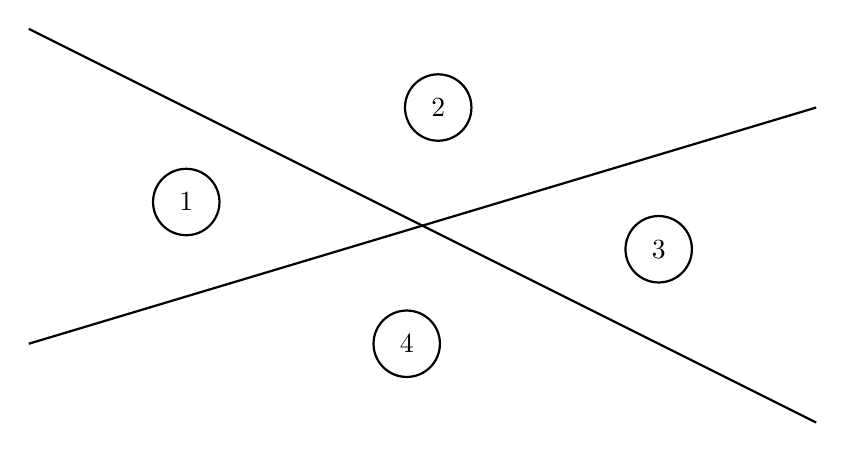
\begin{tikzpicture}[thick]
        \draw (-5,2.5) -- (5,-2.5);
        \draw (-5,-1.5) -- (5,1.5);
        \node[draw,circle,minimum size=24pt,inner sep=0,anchor=center] at (-0.2,-1.5) {$4$};
        \node[draw,circle,minimum size=24pt,inner sep=0,anchor=center] at (3,-0.3) {$3$};
        \node[draw,circle,minimum size=24pt,inner sep=0,anchor=center] at (-3,0.3) {$1$};
        \node[draw,circle,minimum size=24pt,inner sep=0,anchor=center] at (0.2,1.5) {$2$};
    \end{tikzpicture}
\end{center}

然而,这只是两条直线相交的一种\emph{具体情况}。我们怎么知道无论我们如何画这两条线,\emph{总能}得到四个区域?也就是说,我们能否以某种方式结合直线数量 $n = 2$ 这一事实来描述这是\text{如何}发生的?思考一下!

下面是我们的方法。请注意,当我们添加第二条直线时,每个已经存在的区域都会被分成两部分,并且\emph{无论你如何绘制直线},只要我们确保两条直线不平行,结果都是这样。也就是说,如果我们用一条直线将平面分成两个区域,

\begin{center}
    \begin{tikzpicture}[thick]
        \draw (-5,2.5) -- (5,-2.5);
        \node[draw,circle,minimum size=24pt,inner sep=0,anchor=center] at (-3,0.3) {$1$};
        \node[draw,circle,minimum size=24pt,inner sep=0,anchor=center] at (0.2,1.5) {$2$};
    \end{tikzpicture}
\end{center}

然后添加一条新的直线会将每个现有区域分成两部分。这会向整个平面添加两个新的区域,总共四个区域:

\begin{center}
    \begin{tikzpicture}[thick]
        \draw (-5,2.5) -- (5,-2.5);
        \draw [color=red] (-5,-1.5) -- (0,0)  node[midway,below,sloped]{分割区域 1}
        -- (5,1.5) node[midway,above,sloped]{分割区域 2} ;
        \node[draw,circle,minimum size=24pt,inner sep=0,anchor=center,color=red] at (-0.2,-1.5) {$4$};
        \node[draw,circle,minimum size=24pt,inner sep=0,anchor=center,color=red] at (3,-0.3) {$3$};
        \node[draw,circle,minimum size=24pt,inner sep=0,anchor=center] at (-3,0.3) {$1$};
        \node[draw,circle,minimum size=24pt,inner sep=0,anchor=center] at (0.2,1.5) {$2$};
    \end{tikzpicture}
\end{center}

当 $n = 3$ 时呢?在这种情况下,我们需要考虑向具有两条直线和四个区域的图形中添加第三条直线。我们想要提出一个不依赖于线的特定排列的论证,因此我们最终唯一能用的事实是线之间互不平行,且任何交点仅位于两条线(而不是三条或更多)上。不过,就目前而言,查看特定的线条排列会有所帮助,以便我们讨论相同的图形;我们可以利用对这个特定图形的观察来指导我们的一般论证。让我们从下方具有两条直线的图开始,向其中添加第三条线,我们让第三条线的交点都在初始交点``附近''或在图的范围内,这样我们就缩放图形了:

\begin{center}
    \begin{tikzpicture}[thick]
        \draw (-5,2.5) -- (5,-2.5);
        \draw (-5,-1.5) -- (5,1.5);
        \draw [color=red] (-5,1) -- (-1.8085,0.9043) node[midway,below,sloped]{\small 分割区域 1} 
        -- (2.5758,0.7727) node[midway,above,sloped]{\small 分割区域 2}
        -- (5,0.7) node[midway,below,sloped]{\small 分割区域 3};
        \node[draw,circle,minimum size=16pt,inner sep=0,anchor=center] at (-0.2,-1.5) {$4$};
        \node[draw,circle,minimum size=16pt,inner sep=0,anchor=center] at (3,-0.3) {$3$};
        \node[draw,circle,minimum size=16pt,inner sep=0,anchor=center] at (-3,-0.3) {$1$};
        \node[draw,circle,minimum size=16pt,inner sep=0,anchor=center] at (0.2,2) {$2$};
        \node[draw,circle,minimum size=16pt,inner sep=0,anchor=center,color=red] at (-4,1.45) {$5$};
        \node[draw,circle,minimum size=16pt,inner sep=0,anchor=center,color=red] at (0.1,0.45) {$6$};
        \node[draw,circle,minimum size=16pt,inner sep=0,anchor=center,color=red] at (4.61,1.05) {$7$};
    \end{tikzpicture}
\end{center}

很明显现在我们有 $7$ 个区域。我们将第三条线设置为不同的颜色,以便我们可以识别``新''区域出现的位置:一个区域(下方区域,区域 $4$)保持不变,但其他三个区域被一分为二,每个``分割''都会让我们的计数加 $1$(原来有 $1$ 个区域,现在有 $2$ 个)。如果我们以不同的方式绘制这条直线会怎样?

\begin{center}
    \begin{tikzpicture}[thick]
        \draw (-5,2.5) -- (5,-2.5);
        \draw (-5,-1.5) -- (5,1.5);
        \draw [color=red] (0,2.5) -- (-0.8333,0.4167) node[midway,right,sloped,rotate=-90]{\small 分割区域 2} 
        -- (-1.1364,-0.341) node[midway,left,sloped,rotate=-90]{\small 分割区域 1}
        -- (-2,-2.5) node[midway,right,sloped,rotate=-90]{\small 分割区域 4}; 
        \node[draw,circle,minimum size=16pt,inner sep=0,anchor=center] at (-0.2,-1) {$4$};
        \node[draw,circle,minimum size=16pt,inner sep=0,anchor=center] at (3,-0.3) {$3$};
        \node[draw,circle,minimum size=16pt,inner sep=0,anchor=center] at (-3,-0.3) {$1$};
        \node[draw,circle,minimum size=16pt,inner sep=0,anchor=center] at (1,2) {$2$};
        \node[draw,circle,minimum size=12pt,inner sep=0,anchor=center,color=red] at (-0.7,0.05) {$5$};
        \node[draw,circle,minimum size=16pt,inner sep=0,anchor=center,color=red] at (-1.5,1.8) {$6$};
        \node[draw,circle,minimum size=16pt,inner sep=0,anchor=center,color=red] at (-2.5,-1.4) {$7$};
    \end{tikzpicture}
\end{center}

同样的现象再次发生,其中一个区域保持不变,但其他三个区域一分为二。(我们怎么知道没有任何其他区域未绘制在我们这个比例的图形内?这并不像看上去的那么容易回答,值得深刻考虑。)尝试三条线的其他排列方式,并试图说服自己这种情况总会发生;此外,思考一下\emph{为什么}会出现这种情况,以及我们\emph{如何}解释这种情况一定会发生。不过,在给出一般性解释之前,我们先来看另一个小案例。

当 $n = 4$ 时,我们从 $3$ 条直线和 $7$ 个区域的平面开始,然后添加第四条直线,该线不与任何现有线平行,并且不穿过任何现有交点。同样,我们想要提出一个与特定的线条排列无关的论证,但是查看下面的具体图形将有助于引导我们的直觉来提出该论证:

\begin{center}
    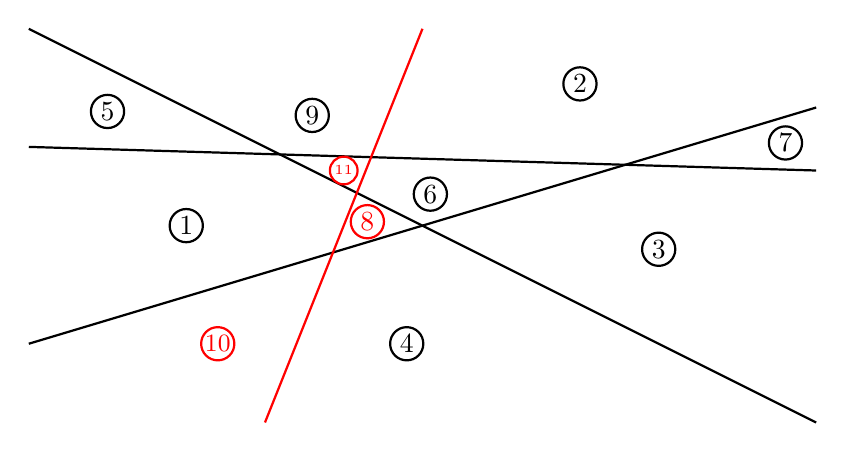
\begin{tikzpicture}[thick]
        \draw (-5,2.5) -- (5,-2.5);
        \draw (-5,-1.5) -- (5,1.5);
        \draw  (-5,1) -- (5,0.7);
        \draw [color=red] (0,2.5) -- (-2,-2.5);
        \node[draw,circle,minimum size=12pt,inner sep=0,anchor=center] at (-0.2,-1.5) {$4$};
        \node[draw,circle,minimum size=12pt,inner sep=0,anchor=center] at (3,-0.3) {$3$};
        \node[draw,circle,minimum size=12pt,inner sep=0,anchor=center] at (-3,0) {$1$};
        \node[draw,circle,minimum size=12pt,inner sep=0,anchor=center] at (2,1.8) {$2$};
        \node[draw,circle,minimum size=12pt,inner sep=0,anchor=center] at (-4,1.45) {$5$};
        \node[draw,circle,minimum size=12pt,inner sep=0,anchor=center] at (-1.4,1.4) {$9$};
        \node[draw,circle,minimum size=10pt,inner sep=0,anchor=center,color=red] at (-1,0.7) {\tiny $11$};
        \node[draw,circle,minimum size=12pt,inner sep=0,anchor=center] at (4.61,1.05) {$7$};
        \node[draw,circle,minimum size=12pt,inner sep=0,anchor=center,color=red] at (-0.7,0.05) {$8$};
        \node[draw,circle,minimum size=12pt,inner sep=0,anchor=center] at (0.1,0.4) {$6$};
        \node[draw,circle,minimum size=12pt,inner sep=0,anchor=center,color=red] at (-2.6,-1.5) {\small $10$};
    \end{tikzpicture}
\end{center}

请注意,三个原始区域保持不变(区域 $3$、区域 $5$ 和区域 $7$),其他四个区域一分为二。你注意到这里存在一个模式吗?似乎对于我们检查过的每个 $n$,添加第 $n$ 条线会使 $n-1$ 个区域保持不变,而其余区域则被一分为二。让我们尝试解释为什么会出现这种情况。请记住,当我们绘制 $n$ 条直线时,我们试图确定出现了多少个区域,因此让我们为该值分配一个``名称'',以便我们可以引用它;假设 $R(n)$ 表示在平面上绘制 $n$ 条直线所创建的区域数,且没有两条线平行,并且没有交点在两条以上的线上。在上面示例中,我们考虑了 $n$ 的较小取值,并研究了添加新的直线时会发生什么变化;也就是说,我们可以通过已知 $R(n - 1)$ 算出 $R(n)$ 的值。让我们整理一下我们的观察结果,以便它们适用于\emph{任意} $n$ 值。

假设我们已知 $R(n)$。(为什么我们可以这样做?对于某个特定的 $n$,我们是否确实知道 $R(n)$ 的特定值?这个值是什么?如何知道的?)假设我们在平面上有一个\emph{任意} $n$ 线图,满足上面题目陈述中给出的两个条件。这些直线创建了多少个区域?是的,正是 $R(n)$。现在,当我们添加第 $(n + 1)$ 条直线时会发生什么?关于这条线以及它如何改变图形,我们可以确定什么?其实,我们真正掌握的唯一信息是:

\begin{enumerate}[label=(\alph*)]
    \item 这条新的直线与现有的 $n$ 条直线中的任何一条都不平行;
    \item 这条新的直线不经过任何现有的交点。
\end{enumerate}

现在,条件 (a) 告诉我们这条新的直线必须与\emph{所有}现有的 $n$ 条直线线相交;平行线不相交,非平行线必然相交于某处。因此,我们必须在图上创建 $n$ 个新的交点。这些交点会与任何现有交点重合吗?不会!这正是条件 (b) 告诉我们的。这两条信息合在一起告诉我们,无论我们如何绘制这条新的直线,只要它满足题目的要求,这条直线上\emph{一定}会出现 $n$ 个``特殊''点。这些特殊点正是新线与现有线的交点。

我们现在想利用这些特殊点来识别图中的新区域。回顾一下我们上面研究的案例:识别新的交点,看看是否可以将它们与新的区域关联起来。也许用圆点标记这些交点并用 $\textbf{×}$ 标记新区域会有所帮助,让它们更容易辨认。我们在下面为你展示了一个示例,其中 $n = 4$。你注意到了什么?你能用这些点来帮助识别添加第 $n$ 条直线后创建了多少新区域吗?思考一下,然后继续阅读。

\begin{center}
    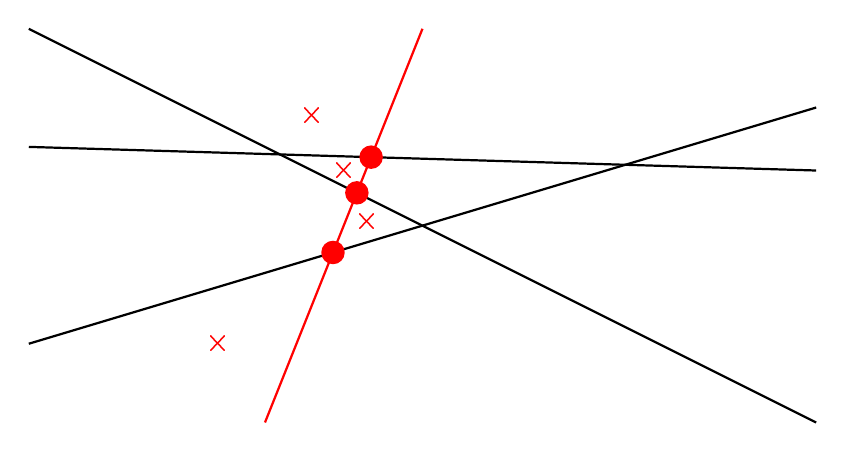
\begin{tikzpicture}[thick]
        \draw (-5,2.5) -- (5,-2.5);
        \draw (-5,-1.5) -- (5,1.5);
        \draw  (-5,1) -- (5,0.7);
        \draw [color=red] (0,2.5) -- (-2,-2.5);
        \node[minimum size=14pt,anchor=center,color=red,very thick] at (-1.4,1.4) {$\textbf{×}$};
        \node[minimum size=14pt,anchor=center,color=red,very thick] at (-1,0.7) {$\textbf{×}$};
        \node[minimum size=14pt,anchor=center,color=red,very thick] at (-0.7,0.05) {$\textbf{×}$};
        \node[minimum size=14pt,anchor=center,color=red,very thick] at (-2.6,-1.5) {$\textbf{×}$};
        \node[fill,circle,inner sep=3pt,color=red] at (-0.6522,0.8696) {};
        \node[fill,circle,inner sep=3pt,color=red] at (-0.8333,0.4167) {};
        \node[fill,circle,inner sep=3pt,color=red] at (-1.1364,-0.341) {};
    \end{tikzpicture}
\end{center}

没错!任意两个相邻新交点之间,都有一条\emph{线段}将一个区域一分为二!剩下的就是确定我们创建了多少个新的此类线段。由于每条线段都将唯一\emph{一个}现有区域一分为二,因此这将准确地告诉我们创建了多少个新区域。我们已知,第 $(n + 1)$ 条直线线创建了 $n$ 个新的交点。想想这些点是如何排列在直线上的。任意两个``连续''点都会创建一条线段,但极点也会创建无限线段(永远延申下去经过这些极点)。总共有多少个?正好是 $n + 1$。(参考上图,$n = 3$。我们看到有 $3$ 个新交点和 $4$ 条新线段,其中两个是无限射线。)这意味着有 $n + 1$ 条线段将区域一分为二,因此我们恰好创建了 $n + 1$ 个新区域!这让我们可以说
\[R(n + 1) = R(n) + n + 1\]
哇,多好的观察啊!我们花了一些时间研究示例并进行了一些几何论证,但最终我们做到了。我们已经确定了这个问题的一些归纳结构;我们发现一个情况如何依赖另一个情况。也就是说,我们发现了 $R(n+1)$ 如何依赖 $R(n)$。这还没有完全解决这个问题,但我们现在已经非常接近了。剩下的就是用类似的表达式替换 $R(n)$,并不断执行此操作,直到达到我们已知的 $R(1) = 2$。观察:

\begin{center}
    \begin{tabular}{rcccccccccc}
        $R(n+1)$ & $=$ &          & &            &     &            &     & $\cancel{R(n-1)}$ & $+$ & $n+1$\\
                 & $=$ &          & &                   &     & $\cancel{R(n-1)}$ & $+$ & $n$ & $+$ & $n+1$\\
                 & $=$ &          & & $\cancel{R(n-2)}$ & $+$ & $(n-1)$           & $+$ & $n$ & $+$ & $n+1$\\
                 & $\vdots$ &     & &  &  &  &  &  &  & \\
                 & $=$ &          & & $\cancel{R(2)}+3$ & $+$ & $\dots$ & $+$ & $n$ & $+$ & $n+1$ \\
                 & $=$ & $R(1)+2$ & $+$ & $3$               & $+$ & $\dots$ & $+$ & $n$ & $+$ & $n+1$ \\
    \end{tabular}
\end{center}

因为我们知道 $R(1) = 2$,所以我们可以说
\[R(n + 1) = 2 + \big(2 + 3 + \dots + n + (n + 1)\big) = 2 + \Bigg(\sum_{k=1}^{n+1}k\Bigg)-1 = 1+\sum_{k=1}^{n+1}k\]
而这正是我们之前研究过的求和公式!(另请注意,我们必须减去 $1$,因为括号中缺少求和的第一项。)回想一下 $\sum_{k=1}^{n} k = \frac{n(n+1)}{2}$,为了表示上面等式中的求和,我们只需将 $n$ 替换为 $n + 1$ 即可。因此,
\[R(n + 1) = 1+\frac{(n+1)(n+2)}{2}\]
我们要进行的最后一步简化是将整个方程中的 $n+1$ 替换为 $n$,因为使用 $R(n)$ 的表达式更有意义(对 $n$ 的值有什么要求?)
\[R(n + 1) = 1+\frac{n(n+1)}{2}\]
最终,我们找到了开头问题的答案!在这个过程中,我们采用了\emph{归纳}技术:我们解释了一个``事实''(即 $R(n + 1)$ 的值)如何\emph{取决于}``前一个事实''(即 $R(n)$ 的值),并使用这些迭代依赖关系进行反向运算,直到达到一个特定的\emph{已知}值,即 $R(1)$。

我们想再次指出,我们在本节中所做的推导和观察只是引导我们的直觉从而得出答案,并不是\emph{严格证明}。问题出在 ``$\dots$'' 身上,省略号不是具体的、``官方''的数学方法来捕获归纳技术背后的归纳过程。此外,我们解决``平面中的线''问题的方法是从 $n - 1$ 条线的图形\emph{开始,构建}一个包含 $n$ 条线的新图;这样可以吗?为什么这实际上告诉了我们有关 $n$ 条线的\emph{任意}图的信息?所有这些图都来自于少了一条线的较小图吗?

在接下来的两章中,我们将学习必要的工具来充分描述我们迄今为止所做事情的严格方法,在那之后的章节中,我们将使用这些工具让数学归纳法变得正式而严谨。不过,现在我们想给出归纳法的启发式定义,并继续研究依赖归纳技术的有趣问题和观察结果。练习这些类型的问题 --- 学习何时识别归纳过程、如何使用它、如何使用该结构来解决问题等等 --- 将在未来非常有帮助,我们不需要深入到数学技术细节。(至少,现在还不需要!)


% !TeX root = ../../../book.tex
\subsection{习题}

\subsubsection*{温故知新}

以口头或书面的形式简要回答以下问题。这些问题全都基于你刚刚阅读的内容,所以如果忘记了具体的定义、概念或示例,可以回去重读相关部分。确保在继续学习之前能够自信地回答这些问题,这将有助于你的理解和记忆!

\begin{enumerate}[label=(\arabic*)]
    \item 归纳过程有哪些特征?
    \item 我们如何证明 $\sum_{k=1}^{n}k = \frac{n(n+1)}{2}$ 是正确的?我们的方法是如何归纳的?(如果你不记得了,请重读第 \ref{sec:section1.4.2} 节!)
    \item 为什么我们可以把上一个问题中提到的求和公式,用 $n+1$ ``替换'' $n$,并且知道它仍然成立?我们也可以将 $n$ 替换为 $n - 1$ 吗?
    \item 通过代数步骤获得前 $n$ 个自然数平方和的最终表达式;也就是说,验证
    \[\frac{1}{3}(n+1)^3-\frac{1}{3}(n+1)-\frac{n(n+1)}{2} = \frac{1}{6}n(n+1)(2n+1)\]
    \item 试着回忆一下向平面中添加第 $(n+1)$ 条直线正好会创建 $n+1$ 个新区域的论点。你能为朋友证明这个论点并说服他/她它是有效的吗?
    \item 求前 $n$ 个自然数的平方和,为什么不能把前 $n$ 个自然数之和的公式平方呢?为什么这是错误的?
\end{enumerate}

\subsubsection*{小试牛刀}

尝试回答以下问题。这些题目要求你实际动笔写下答案,或(对朋友/同学)口头陈述答案。目的是帮助你练习使用新的概念、定义和符号。题目都比较简单,确保能够解决这些问题将对你大有帮助!

\begin{enumerate}[label=(\arabic*)]
    \item 在平面中画 $5$ 条直线(满足原题的两个条件)并验证是否有 $16$ 个区域。你还能验证 $6$ 条线产生 $22$ 个区域吗?
    \item 给出序列 $1, 2, 3, 4, \dots , 100$ 的另一种解释,而不仅仅是从 $1$ 到 $100$ 的所有自然数。(回想一下我们给出的例子:$1$ 到 $100$ 之间所有英文拼写中不含字母``i''的数字。)
    \item 提出一个将 $(n + 1)^4$ 与 $n^4$ 联系起来的代数表达式,就像我们对立方所做的那样。\\ 
    (\textbf{挑战题:}你能为刚刚推导出的表达式给出\emph{几何}解释吗?)
    \item \textbf{挑战题:}让我们将``平面上的线''这题提升一个维度!考虑三维空间中有 $n$ 个平面。会创建多少个区域?假设没有两个平面平行,并且没有三个或以上平面相交于一条直线。(想想这两个条件如何直接类比于``线''那题的给定条件。)
\end{enumerate}

\newpage
% !TeX root = ../../../book.tex
\section{定义归纳}

为了阐明数学归纳法这一证明技术,我们需指出:前一节的示例依赖于问题结构的直观理解来给出``解''——此处\emph{解}上加引号表明尚未严格证明。由此引出核心问题:若我们被要求直接验证先前推导的公式,而未曾通过直观过程获得它,仅被告知其正确性,该如何证明?这正是当前面临的情形,除非告知者采用了与我们相同的直观论证。

假设一位持怀疑态度的朋友声称:``我听说计算前 $n$ 个自然数平方和的公式是 $\frac{1}{6}n(n+1)(2n+1)$。验证前两个数完全吻合,因此它必然正确,可以确信无疑!''作为理性的思考者兼好友,你回应道:``我也听闻此公式,但需确保它对所有自然数均成立。''如何展开验证?朋友所言非虚,前几项确实``完美匹配'':
\begin{align*}
    1^2 &= \enspace 1 = \frac{1}{6}(1)(2)(3) \\
    1^2 + 2^2 &= \enspace 5 = \frac{1}{6}(2)(3)(5) \\
    1^2 + 2^2 + 3^2 &= 14 = \frac{1}{6}(3)(4)(7) \\
    1^2 + 2^2 + 3^2 + 4^2 &= 30 = \frac{1}{6}(4)(5)(9)
\end{align*}
如果我们愿意的话,甚至可以手动检验更大的 $n$ 值:
\[1^2 + 2^2 + 3^2 + 4^2 + 5^2 + 6^2 + 7^2 + 8^2 + 9^2 + 10^2 = 385 = \frac{1}{6}(10)(11)(21)\]
然而该公式宣称对\emph{任意} $n$ 成立。自然数有\emph{无穷}多个,逐一验证从数学和时间上皆不可行——无论检验多少独立的 $n$ 值,总会有更大的 $n$ 值未经验证。我们如何\emph{确知}公式不会在某个较大的 $n$ 值失效?这要求一种数学上\emph{高效}的方法,能以有限步骤验证所有情形。为此我们引入初步构想(后续将严格表述的数学归纳法),从原理层面说明其运作机制。

% !TeX root = ../../../book.tex
\subsection{多米诺骨牌类比}

假设我们有一副特殊的多米诺骨牌,它包含无穷多张骨牌!每张骨牌可以书写任意内容,而非标准的点数。这些骨牌沿无限延伸的桌面排列成无限长的一行。从侧面观察时,每张骨牌下方标有位置标签:

\begin{center}
    \begin{tikzpicture}
        \foreach \x in {1,...,5}
        {
            \pic [fill=white] at (\x, 0, 0) {annotated cuboid={width=3, height=30, depth=10}};
            \node[below] at (\x, -3){\tiny $n=\x$};
        }
        \node[anchor=center] at (6.5, -1.5){\LARGE $\dots \cdot$};
        % \pic [very thick,densely dashed,draw=blue] at (5,0) {annotated cuboid={width=30, height=5, depth=10, opacity=0.2}};
    \end{tikzpicture}
\end{center}

对于这个特定的例子,我们需要验证公式
\[\sum_{k=1}^{n}k^2 = \frac{1}{6}n(n+1)(2n+1)\]
为此,设想每张多米诺骨牌记载一个特定``事实''。具体来说,我们可以想象第一张多米诺骨牌上写有表达式
\[\sum_{k=1}^{1}k^2 = \frac{1}{6}(1)(1)(3)\]
第二张多米诺骨牌上写有表达式
\[\sum_{k=1}^{2}k^2 = \frac{1}{6}(2)(3)(5)\]
推而广之,第 $n$ 张骨牌写有如下``事实'':
\[\sum_{k=1}^{n}k^2 = \frac{1}{6}n(n+1)(2n+1)\]
由于多米诺骨牌具有连锁倾倒的特性,我们约定骨牌倒下即表示其记载的``事实''是\emph{真实命题}。由此将多米诺骨牌的物理解释与公式有效性的数学解释联系起来。

我们已手动验证 $n=1$ 的情形:$1^2=\frac{1}{6}(1)(2)(3)$,故第一张骨牌记载的命题为真,必将倒下。同理验证 $n=2$ 后,第二张骨牌也会倒下:

\begin{center}
    \begin{tikzpicture}
        \foreach \x in {1,2}
        {
            \pic [fill=white, rotate=-30, anchor=south] at (\x, -0.15, 0) {annotated cuboid={width=3, height=32, depth=10}};
            \node[below] at (\x-1.5, -3){\tiny $n=\x$};
        }
        \foreach \x in {3,4,5}
        {
            \pic [fill=white] at (\x, 0, 0) {annotated cuboid={width=3, height=30, depth=10}};
            \node[below] at (\x, -3){\tiny $n=\x$};
        }
        \node[anchor=center] at (6.5, -1.5){\LARGE $\dots \cdot$};
        % \pic [very thick,densely dashed,draw=blue] at (5,0) {annotated cuboid={width=30, height=5, depth=10, opacity=0.2}};
    \end{tikzpicture}
\end{center}
然而,若继续逐个检验,又会陷入原先的困境——我们不可能验证\emph{每张}骨牌。真正的需求是捕捉多米诺效应的精髓:一张骨牌倒下将触发下一张倒下。这要求我们建立相邻骨牌所载``事实''的数学关联。

让我们看看前两张多米诺骨牌的情况。既然知道骨牌 $1$ 倒下,我们能否在不重写所有求和项的情况下确保骨牌 $2$ 倒下?两块骨牌上的陈述有何关联?每个陈述都是自然数的平方和,且第二张骨牌的陈述正好多出一项。因此,利用骨牌 $1$ 上已知的\emph{真实陈述},可以\emph{验证}骨牌 $2$ 上陈述的真实性:
\[\sum_{k=1}^{2}k^2 = 1^2+2^2=1+2^2=5=\frac{1}{6}(2)(3)(5)\]
尽管节省的唯一``工作''只是免于计算 $1^2=1$,但让我们在更大数字上应用此过程以凸显其优势。\emph{假设}骨牌 $10$ 已经倒下(其求和的完整验证已在前文给出),这意味着我们\emph{知道}
\[\sum_{k=1}^{10}k^2 =\frac{1}{6}(10)(11)(21)=285\]
是一个\emph{真实陈述}。利用它来验证骨牌 $11$ 的陈述:
\[\sum_{k=1}^{11}k^2 =\frac{1}{6}(11)(12)(23)\]
骨牌 $11$ 上的求和公式有 $11$ 项,前 $10$ 项正是骨牌 $10$ 上的求和!因此只需分离第 $11$ 项并代入已知结果:
\begin{align*}
    \sum_{k=1}^{11}k^2 &= (1^2+2^2+\dots+10^2)+11^2\\
    &=\sum_{k=1}^{10}k^2+11^2\\
    &=385+121\\
    &=506\\
    &=\frac{1}{6}3036=\frac{1}{6}(11)(12)(23)
\end{align*}
节省的工作量显而易见!既然已知前 $10$ 项之和,何必重新计算?

现在设想对\emph{所有} $n$ 值\emph{同时}实施此过程!若能证明每当骨牌 $n$ 倒下,骨牌 $(n + 1)$ \emph{必然}倒下,这意味着什么?回顾无穷骨牌序列:已知骨牌 $1$ 因手动检验而倒下,加之``骨牌 $n$ 撞倒骨牌 $(n + 1)$''的普适性验证,可推得骨牌 $1$ 撞倒骨牌 $2$,骨牌 $2$ 撞倒骨牌 $3$,骨牌 $3$ 撞倒骨牌 $4$,…… 如此传递下去,整列骨牌终将全部倒下!本质上,整个过程可归结为\emph{两步}:

\begin{enumerate}[label=(\arabic*)]
    \item 确保第一张骨牌倒下;
    \item 确保每张骨牌都能撞倒下一张骨牌。
\end{enumerate}
仅凭这两步,便能\emph{保证}所有骨牌倒下,从而\emph{证明}每个公式对\emph{任意}自然数 $n$ 成立。

我们已经完成步骤 (a),现在需要完成步骤 (b)。此前已针对特定案例(骨牌 $1$ 撞倒骨牌 $2$、骨牌 $10$ 撞倒骨牌 $11$)执行了此操作,现在将其推广到任意 $n$ 值。我们\emph{假设}:对于某个\emph{特定}但\emph{任意}的 $n$,多米诺骨牌 $n$ 会倒下,这意味着方程
\[\sum_{k=1}^{n}k^2=\frac{1}{6}n(n+1)(2n+1)\]
为\emph{真实陈述}。现在需将其关联到骨牌 $(n+1)$ 的陈述,并应用上述等式信息。将 $n+1$ 项的和拆分为 $n$ 项和与末项:
\[\sum_{k=1}^{n+1}k^2 = (1^2+2^2+\dots+n^2+(n+1)^2)=\sum_{k=1}^{n}k^2+(n+1)^2\]
根据骨牌 $n$ 倒下的假设(即其命题为真),可得
\[\sum_{k=1}^{n+1}k^2 = \frac{1}{6}n(n+1)(2n+1)+(n+1)^2\]
这与骨牌 $(n+1)$ 的命题是否一致?骨牌 $(n+1)$ 的``事实''与骨牌 $n$ 类似,只是将``$n$''替换为``$n + 1$'':
\[\sum_{k=1}^{n+1}k^2 = \frac{1}{6}\big(n+1\big)\big((n+1)+1\big)\big((2(n+1)+1)\big)=\frac{1}{6}(n+1)(n+1)(2n+3)\]
目前还不清楚我们推导出的表达式是否实际上等于上面的式子。我们可以尝试化简该表达式,并将其分解为与上面表达式``类似''的新表达式,但展开两个表达式并比较所有项可能会更容易。(这基于这样的一般思想:展开因式分解后的多项式比进行因式分解要容易得多。)对于第一个表达式,我们有
\begin{align*}
    \frac{1}{6}n(n + 1)(2n + 1) + (n + 1)^2 &=\frac{1}{6}n(2n^2 + 3n + 1) + (n^2 + 2n + 1)\\
    &= \frac{1}{3}n^3 + \frac{1}{2}n^2 + \frac{1}{6}n + n^2 + 2n + 1 \\
    &= \frac{1}{3}n^3 + \frac{3}{2}n^2 + \frac{13}{6}n + 1
\end{align*}
对于第二个表达式,我们有
\begin{align*}
    \frac{1}{6}(n+1)(n + 2)(2n + 3) &=\frac{1}{6}(n+1)(2n^2 + 7n+6)\\
    &= \frac{1}{6}\big[(2n^3 + 7n^2 + 6n) + (2n^2 + 7n + 6)\big] \\
    &= \frac{1}{3}n^3 + \frac{3}{2}n^2 + \frac{13}{6}n + 1
\end{align*}
可见两式相等!此外,请注意,这比尝试整理其中一个表达式并将其``变形''为另一个表达式要容易得多。我们通过展开两式并最终得到相同的表达来证明它们是相同的。现在,让我们回顾并总结我们所取得的成果:
\begin{enumerate}
    \item 我们将证明公式
    \[\sum_{k=1}^{n+1}k^2 = \frac{1}{6}n(n+1)(2n+1)+(n+1)^2\]
    对于\emph{所有} $n$ 值成立类比为推倒无穷多的多米诺骨牌。
    \item 通过手工计算验证骨牌 $1$ 的命题成立,骨牌 $1$ 倒下;
    \item \emph{假设}骨牌 $n$ 的命题为真,由骨牌 $n$ 命题成立推出骨牌 $(n+1)$ 命题成立,从而证明骨牌 $n$ 会撞倒骨牌 $(n+1)$。
    \item 由此保证所有骨牌都会倒下,因此公式对\emph{所有} $n$ 都成立。
\end{enumerate}
此方法是否严谨?是否已\emph{严格证明}公式对所有自然数 $n$ 都成立?若存在 $n$ 使得公式失效,这对多米诺骨牌体系意味着什么?

请记住,这里的多米诺骨牌类比只是理解归纳法工作原理的一个直观指引,并非建立在严格的数学基础之上。建立严格的数学基础将是接下来几章的目标。现在,让我们回顾本章讨论的另一个例子:直线划分平面区域。同样,在推导公式 $R(n)$ 时使用省略号显得繁琐,我们希望避免这种做法。让我们尝试将多米诺骨牌类比应用于此问题。

设想我们定义 $R(n)$ 为 $n$ 条直线在平面上划分出的不同区域的数量,这些直线满足互不平行且任意三条(或更多)直线不共点。进一步设想,我们在代表第 $n$ 步的骨牌上写下``$R(n) = 1 + \frac{n(n+1)}{2}$''这一``事实''。能否按照与之前相同的逻辑来验证所有骨牌都会倒下?

首先,需要验证骨牌 $1$ 是否会倒下。这等同于验证命题``$R(1) = 1+\frac{1(2)}{2} = 1+1 = 2$''是否成立。这显然成立,正如我们之前验证过的:一条直线将平面划分为两个区域。其次,需要证明对于\emph{任意} $n$,第 $n$ 块骨牌倒下必定导致第 $(n + 1)$ 块骨牌倒下。也就是说,我们\emph{假设}``$R(n) = 1 + \frac{n(n+1)}{2}$''对某个特定的 $n$ 成立,然后\emph{证明}``$R(n + 1) = 1 + \frac{(n+1)(n +2)}{2}$''也必然成立。如何证明?沿用之前的思路,建立 $R(n + 1)$ 与 $R(n)$ 的关系。向\emph{任意}满足条件的 $n$ 条直线的图形中添加一条新直线,通过几何分析,我们得到关系式 $R(n+1) = R(n) + n + 1$。利用此关系以及第 $n$ 块骨牌倒下的假设,可得:
\[R(n + 1) = R(n) + n + 1 = 1 +\frac{n(n+1)}{2}+ n + 1\]
这个结果是否与骨牌 $(n + 1)$ 上的表达式一致?通过化简比较即可验证:
\[1 +\frac{n(n+1)}{2}+ n + 1=2+n+\frac{n^2+n}{2} = \frac{1}{2}n^2+\frac{3}{2}n+2\]
以及
\[1 + \frac{(n+1)(n +2)}{2} = 1+\frac{n^2+3n+2}{2} =  \frac{1}{2}n^2+\frac{3}{2}n+2\]
结果完全相同!因此,我们证明了对于\emph{任意} $n$,骨牌 $n$ 倒下\emph{必然}导致骨牌 $(n+1)$ 倒下。

思考一下,使用这种``多米诺骨牌技术''进行的证明,与我们之前为推导该公式所采用的方法有何不同?我们在本节中是否使用了省略号?为何这种证明方式更优?我们是否曾用多米诺骨牌归纳技术来推导公式本身?


% !TeX root = ../../../book.tex
\subsection{其他类比}

多米诺骨牌类比非常流行,但它并非描述归纳法工作方式的唯一途径。根据阅读材料或交流对象的不同,你可能会接触到不同的类比或其他形式的阐释。在此,我们将介绍两种常见的类比。思考这些类比在本质上的相通之处,将有助于深化你对归纳法的理解(至少基于我们已有的探讨)。

\subsubsection*{神奇的数学猴子 Mojo}

想象一架直冲云霄的无穷天梯,梯级按 $1, 2, 3$ 的顺序无限延伸。我们的朋友 Mojo 伫立在梯子旁。这只聪慧的猴子痴迷数学,更拥有神奇的能力——他能真正攀爬这架无穷天梯!

Mojo 踏上某一级阶梯,即代表与该数字对应的事实成立。如何确保他爬完整架梯子?逐一检查每级阶梯效率低下:我们需要先确认他抵达第 $1$ 级,再验证他到达第 $2$ 级,接着是第 $3$ 级……如此往复。更高效的方法是在 Mojo 攀爬前确认两点:第一,他是否踏上起点(即第 $1$ 级)?若是,那就太好了!第二,阶梯间距是否足够近,使他无论身处何处,\emph{总能}登上下一级?若满足此条件,那就更棒了!这些要求与多米诺骨牌类比中的条件完全一致。要确保 Mojo 抵达\emph{每一级}阶梯,只需确认他踏上第 $1$ 级并能持续迈向下一级。

\subsubsection*{归纳鸭 Doug}

再来认识一下 Doug ——一只酷爱面包的鸭子。为了觅食,他会造访数学镇归纳街上每户人家的院子。这些院子沿街排列,门牌号依次为 $1, 2, 3, \dots$。

Doug 从 $1$ 号院子开始搜寻面包。一无所获的他饥肠辘辘,便转向隔壁的 $2$ 号院子。再次空手而归的他只能继续前行。此时已知 $1$ 号院无面包,因此唯一的选择只能是隔壁的 $3$ 号院……我想你已预见到了结局。

如果我们追踪 Doug 的行迹,我们或许好奇他是否终将踏足每个院子。假设已知\emph{所有院子均无面包},这意味着每当 Doug 身处某院,必将前往隔壁院子继续寻找。由此,他必定会挨家挨户探索!换言之,无论你住在编号多大的房子,终将在某一刻目睹 Doug 在你的后院徘徊(遗憾的是,他永远腹中空空——可怜的 Doug!)。


% !TeX root = ../../../book.tex
\subsection{总结}

回顾前两个示例的工作及我们的类比,可以发现每个问题都具有特定的\emph{结构}:某个``事实''依赖于``前一个事实''。对于立方数,我们找到了用 $n^3$ 表示 $(n + 1)^3$ 的方法;对于平面分割问题,我们刻画了向 $n$ 条直线的图形添加新直线时新增的区域个数。基于这些观察,我们反复应用已知关系,直至抵达一个可验证的``基础事实''——通常对应较小的 $n$ 值(两例中均为 $n = 1$)。这一过程使我们能够推导出适用于\emph{任意} $n$ 的通用公式或表达式。

尽管这项工作对公式推导至关重要且富有启发性,但它本身\emph{不足以证明}公式的有效性。在进行上述工作时,我们发现了归纳过程的存在,并利用其结构推导了相关表达式。这实际上有两个好处:不仅发现了待证公式,还让我们意识到采用\emph{数学归纳法}进行严格证明的可行性。

实际的``归纳证明''包含两个核心步骤:首先,验证公式在某个``起始值''成立;其次,\emph{假设}公式对某个特定 $n$ 成立,并以此证明其对 $n + 1$ 必然成立。完成这两步后,我们即可断言``所有多米诺骨牌都会倒下''——公式对所有相关 $n$ 值都成立。

\subsubsection*{一个问题:梯子的``尽头''是什么?}

你可能仍存疑虑,我们尝试在此预测你的担忧。(之所以提及这一点,是因为这是一个常见疑问。若你\emph{未曾}考虑这一点,请试着想象其来源。)你或许会说:``等等,现在我明白 Mojo 如何攀登天梯了,但他如何真正\emph{抵达顶端}呢?这是个无穷阶梯,对吗?那他永远无法到达终点……不是吗?''

某种意义上,你是对的。既然这个神奇阶梯将\emph{永远}延伸,它便没有真正的终点,Mojo 永无法抵达``顶端''。然而,这并非关键;我们不在意任何``\emph{顶端}''(不仅仅是因为\emph{不存在}顶端),只需确认 Mojo 能踏足\emph{每一个}台阶。他不必凌驾所有台阶立于顶端俯视来路——那不是目的!知道 Mojo 实际上到达了\emph{每一个可能的}阶梯。他不必超越所有人,站在梯子的顶端,俯视自己的来路。那不是目标!

不妨这样思考:假设你对某个待证事实抱有浓厚兴趣,例如
\[\text{事实\ } \#18,458,789,572,311,000,574,003 \text{\ (具体数值无关紧要)}\]
它对应遥不可及的台阶,而你只关心 Mojo 能否抵达。他会到达吗?他当然会!这或许需要漫长的时光(多少步呢?),但这在猴子与梯子的神奇世界,谁又在乎时间呢?你知道他终将抵达,这就够了。试想每个事实在神奇世界里都有专属关注者,每位关注着都将因 Mojo 踏足其关切之阶而欣喜。无人在意他能否登顶——那并非焦点。与此同时,在现实世界中,我们因\emph{所有}关注者终将如愿而欣慰。无限攀登的过程被简化为两步:仅凭此两步,我们便确信阶梯的\emph{每一级}皆可达,每个编号的事实皆成立。

亦可类比多米诺骨牌:我们是否在意骨牌链存在``终点'',最终撞上墙壁?当然不。骨牌链将永续延伸,每张牌终会倒下,时间长短无关紧要。同理,我们知晓 Doug 终将抵达\emph{所有}院子——何时抵达\emph{某个}院子无关紧要,唯有抵达\emph{全部}院子方为关键。


% !TeX root = ../../../book.tex
\subsection{习题}\label{sec:section2.3.4}

\subsubsection*{温故知新}

以口头或书面的形式简要回答以下问题。这些问题全都基于你刚刚阅读的内容,所以如果忘记了具体的定义、概念或示例,可以回去重读相关部分。确保在继续学习之前能够自信地回答这些问题,这将有助于你的理解和记忆!

\begin{enumerate}[label=(\arabic*)]
    \item 多米诺骨牌、Mojo 和 Doug 类比是如何等价的?你能给出``函数''来描述它们的关系,将一种类比转换成另一种类比吗?
    \item 找一个没学过数学归纳法的朋友,试着向他描述一下数学归纳法。你发现自己使用了其中的类比吗?有帮助吗?
    \item 为什么我们对立方体的研究未能证明求和公式?为什么我们还需要完成所有这些工作?
    \item 想想多米诺骨牌的类比。多米诺骨牌永远持续下去是一个问题吗?这是否意味着有些多米诺骨牌永远不会倒下?尝试用类比来描述这意味着什么。
\end{enumerate}

\subsubsection*{小试牛刀}

尝试回答以下问题。这些题目要求你实际动笔写下答案,或(对朋友/同学)口头陈述答案。目的是帮助你练习使用新的概念、定义和符号。题目都比较简单,确保能够解决这些问题将对你大有帮助!

\begin{enumerate}[label=(\arabic*)]
    \item 通过归纳步骤来证明该公式
    \[\sum_{k=1}^{n}k = \frac{n(n+1)}{2}\]
    \item 通过归纳步骤来证明该公式
    \[\sum_{k=1}^{n}2k-1 = n^2\]
    \item 通过归纳步骤来证明该公式
    \[\sum_{k=1}^{n}k^3 = \Bigg(\frac{n(n+1)}{2}\Bigg)^2\]
    \item 假设我们有一系列由自然数索引的事实。我们使用表达式 ``$P(n)$'' 表示第 $n$ 个事实。
    \begin{enumerate}[label=(\alph*)]
        \item 如果我们想证明对于每个自然数 $n$,\emph{每个}事实都为真,我们应该怎么做呢?
        \item 如果我们想证明只有 $n$ 为\emph{偶数}时对应的陈述才为真,那该怎么办?我们能做到吗?你能用我们给出的一个类比稍作修改来描述你的方法吗?
        \item 如果我们想证明只有 $n$ 大于等于 $4$ 时才对应的陈述才为真,那该怎么办?我们能做到吗?你能用我们给出的一个类比稍作修改来描述你的方法吗?
    \end{enumerate}
\end{enumerate}


\newpage
% !TeX root = ../../../book.tex
\section{另外两个(不同的)例子} \label{sec:section2.4}

本节有两个主要目的。首先,我们旨在避免读者产生归纳法仅适用于证明\emph{数值公式}(如涉及数字或多项式)的误解。归纳法的应用远比这广泛得多!特别是接下来的例子将证明:某些抽象性质对于给定情境中的任意``规模''均成立。我们会看到这仍属于``归纳''的范畴,同时也能观察到其与先前例子的区别。此外,这些例子还揭示了一个重要现象:有时推动多米诺骨牌需要掌握``更多信息''。在之前的案例中,仅需确认骨牌 $n$ 倒下,即可\emph{确保}骨牌 $n + 1$ 随之倒下。但在本节的示例中,我们可能需要了解前几个骨牌的状态。通过这两个例子,我们将总结其与前述多米诺骨牌模型的差异,并预览适用于此类情况的、更通用的归纳技术定义。

% !TeX root = ../../../book.tex
\subsection{多米诺与密铺} \label{sec:section2.4.1}

这个示例比前两个稍显复杂。我们最终仍将证明某个数值公式,但问题本身比单纯操纵代数表达式更直观。此外,在开始阶段我们会注意到一个有趣的现象:必须先解决几个``小案例'',才能推广方法。这将是我们首次探讨如何调整归纳技术以适应其他情况。

我们要回答的问题可以表述如下:

\begin{quote}
    给定一个由 $2 \times n$ 个方格组成的棋盘,有多少种不同的方式能用多米诺骨牌完全覆盖(密铺)该棋盘?覆盖时每个方格必须被有且仅有一块多米诺骨牌覆盖。
\end{quote}
例如,以下是正确的密铺:

\begin{center}
    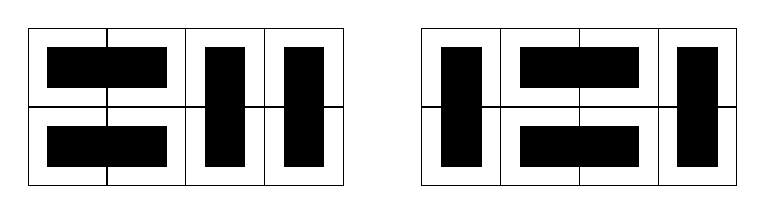
\begin{tikzpicture}[x=1.0cm, y=1.0cm]
        \foreach \y in {0,1} {
            \foreach \x in {0,...,3} {
                \draw (0+\x ,0+\y) rectangle ++ (1,1);
            }
        }

        \draw[fill, black] (0.25 ,0.25) rectangle ++ (1.5,0.5);
        \draw[fill, black] (0.25 ,1.25) rectangle ++ (1.5,0.5);
        \draw[fill, black] (2.25 ,0.25) rectangle ++ (0.5,1.5);
        \draw[fill, black] (3.25 ,0.25) rectangle ++ (0.5,1.5);

        \foreach \y in {0,1} {
            \foreach \x in {0,...,3} {
                \draw (5+\x ,0+\y) rectangle ++ (1,1);
            }
        }

        \draw[fill, black] (5+1.25 ,0.25) rectangle ++ (1.5,0.5);
        \draw[fill, black] (5+1.25 ,1.25) rectangle ++ (1.5,0.5);
        \draw[fill, black] (5+0.25 ,0.25) rectangle ++ (0.5,1.5);
        \draw[fill, black] (5+3.25 ,0.25) rectangle ++ (0.5,1.5);
    \end{tikzpicture}
\end{center}
而以下\emph{不}是正确的密铺:

\begin{center}
    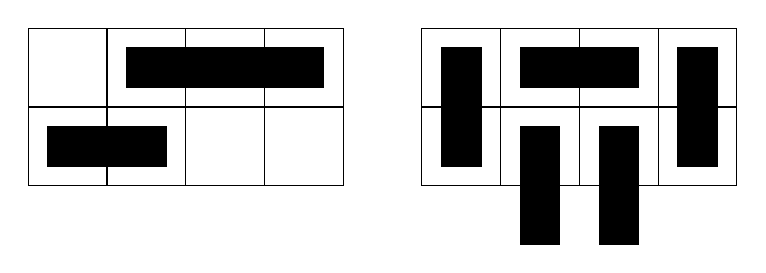
\begin{tikzpicture}[x=1.0cm, y=1.0cm]
        \foreach \y in {0,1} {
            \foreach \x in {0,...,3} {
                \draw (0+\x ,0+\y) rectangle ++ (1,1);
            }
        }

        \draw[fill, black] (0.25 ,0.25) rectangle ++ (1.5,0.5);
        \draw[fill, black] (1.25 ,1.25) rectangle ++ (1.5,0.5);
        \draw[fill, black] (2.25 ,1.25) rectangle ++ (1.5,0.5);

        \foreach \y in {0,1} {
            \foreach \x in {0,...,3} {
                \draw (5+\x ,0+\y) rectangle ++ (1,1);
            }
        }

        \draw[fill, black] (5+1.25 ,1.25) rectangle ++ (1.5,0.5);
        \draw[fill, black] (5+1.25 ,-0.75) rectangle ++ (0.5,1.5);
        \draw[fill, black] (5+2.25 ,-0.75) rectangle ++ (0.5,1.5);
        \draw[fill, black] (5+0.25 ,0.25) rectangle ++ (0.5,1.5);
        \draw[fill, black] (5+3.25 ,0.25) rectangle ++ (0.5,1.5);
    \end{tikzpicture}
\end{center}

与之前一样,先观察前几种情形($n = 1, 2, 3$ 等),尝试寻找规律。在继续阅读之前,建议先自行思考!

当 $n = 1$ 时,棋盘形状恰好与一块多米诺骨牌相同,因此仅有一种密铺方式。用 $T(n)$ 表示 $2 \times n$ 棋盘的密铺数,故 $T(1) = 1$。

\begin{center}
    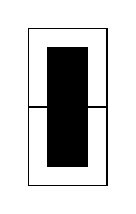
\begin{tikzpicture}[x=1.0cm, y=1.0cm]
        \draw (0,0) rectangle ++ (1,1);
        \draw (0,1) rectangle ++ (1,1);
        \draw[fill, black] (0.25 ,0.25) rectangle ++ (0.5,1.5);
    \end{tikzpicture}
\end{center}

当 $n = 2$ 时,$2 \times 2$ 棋盘有两种不同的密铺方式,此时棋盘的方向很重要,因此 $T(2) = 2$。

\begin{center}
    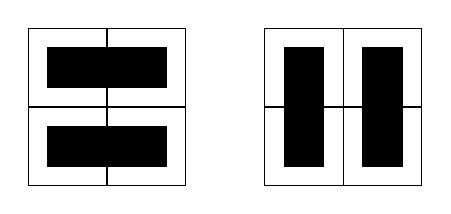
\begin{tikzpicture}[x=1.0cm, y=1.0cm]
        \foreach \y in {0,1} {
            \foreach \x in {0,1} {
                \draw (0+\x ,0+\y) rectangle ++ (1,1);
            }
        }

        \draw[fill, black] (0.25 ,0.25) rectangle ++ (1.5,0.5);
        \draw[fill, black] (0.25 ,1.25) rectangle ++ (1.5,0.5);

        \foreach \y in {0,1} {
            \foreach \x in {0,1} {
                \draw (3+\x ,0+\y) rectangle ++ (1,1);
            }
        }

        \draw[fill, black] (3+0.25 ,0.25) rectangle ++ (0.5,1.5);
        \draw[fill, black] (3+1.25 ,0.25) rectangle ++ (0.5,1.5);
    \end{tikzpicture}
\end{center}

当 $n = 3$ 时,通过枚举可得 $T(3) = 3$。

\begin{center}
    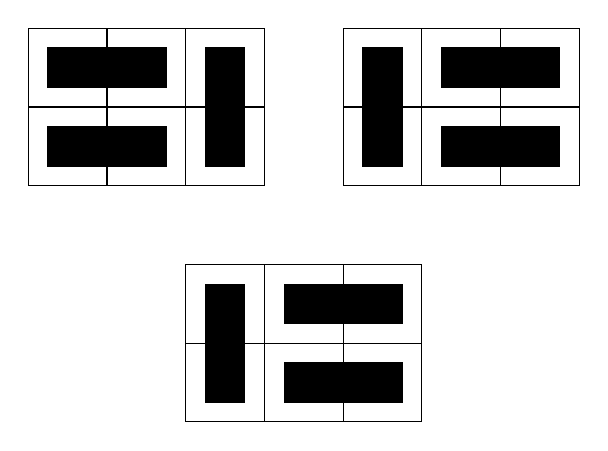
\begin{tikzpicture}[x=1.0cm, y=1.0cm]
        \foreach \y in {0,1} {
            \foreach \x in {0,1,2} {
                \draw (0+\x ,0+\y) rectangle ++ (1,1);
            }
        }

        \draw[fill, black] (0.25 ,0.25) rectangle ++ (1.5,0.5);
        \draw[fill, black] (0.25 ,1.25) rectangle ++ (1.5,0.5);
        \draw[fill, black] (2.25 ,0.25) rectangle ++ (0.5,1.5);

        \foreach \y in {0,1} {
            \foreach \x in {0,1,2} {
                \draw (4+\x ,0+\y) rectangle ++ (1,1);
            }
        }

        \draw[fill, black] (4+1.25 ,0.25) rectangle ++ (1.5,0.5);
        \draw[fill, black] (4+1.25 ,1.25) rectangle ++ (1.5,0.5);
        \draw[fill, black] (4+0.25 ,0.25) rectangle ++ (0.5,1.5);

        \foreach \y in {0,1} {
            \foreach \x in {0,1,2} {
                \draw (2+\x ,-3+\y) rectangle ++ (1,1);
            }
        }

        \draw[fill, black] (2+1.25 ,-3+0.25) rectangle ++ (1.5,0.5);
        \draw[fill, black] (2+1.25 ,-3+1.25) rectangle ++ (1.5,0.5);
        \draw[fill, black] (2+0.25 ,-3+0.25) rectangle ++ (0.5,1.5);
    \end{tikzpicture}
\end{center}

再看 $n=4$ 的情形,可验证 $T(4)=5$。

\begin{center}
    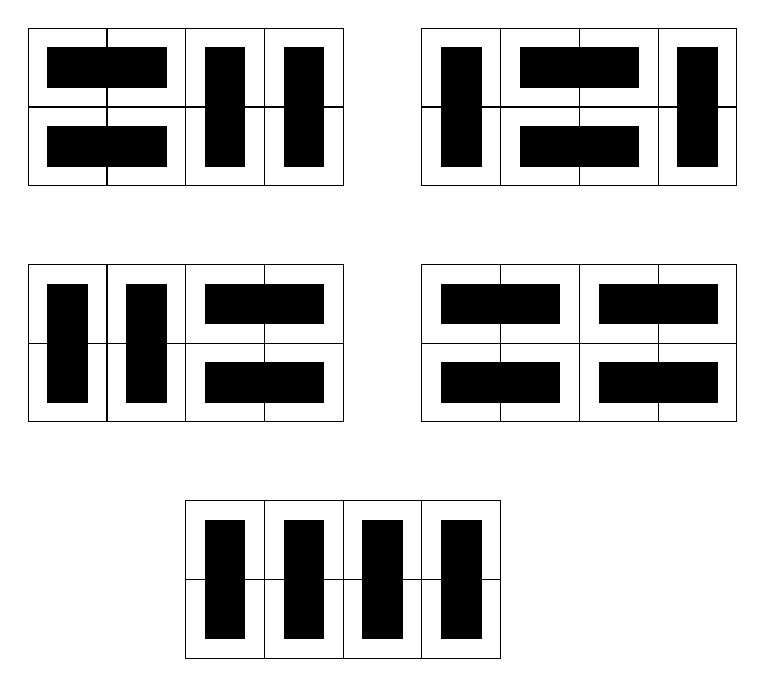
\begin{tikzpicture}[x=1.0cm, y=1.0cm]
        \foreach \y in {0,1} {
            \foreach \x in {0,...,3} {
                \draw (0+\x ,0+\y) rectangle ++ (1,1);
            }
        }

        \draw[fill, black] (0.25 ,0.25) rectangle ++ (1.5,0.5);
        \draw[fill, black] (0.25 ,1.25) rectangle ++ (1.5,0.5);
        \draw[fill, black] (2.25 ,0.25) rectangle ++ (0.5,1.5);
        \draw[fill, black] (3.25 ,0.25) rectangle ++ (0.5,1.5);

        \foreach \y in {0,1} {
            \foreach \x in {0,...,3} {
                \draw (5+\x ,0+\y) rectangle ++ (1,1);
            }
        }

        \draw[fill, black] (5+1.25 ,0.25) rectangle ++ (1.5,0.5);
        \draw[fill, black] (5+1.25 ,1.25) rectangle ++ (1.5,0.5);
        \draw[fill, black] (5+0.25 ,0.25) rectangle ++ (0.5,1.5);
        \draw[fill, black] (5+3.25 ,0.25) rectangle ++ (0.5,1.5);

        \foreach \y in {0,1} {
            \foreach \x in {0,...,3} {
                \draw (0+\x ,-3+\y) rectangle ++ (1,1);
            }
        }

        \draw[fill, black] (2.25 ,-3+0.25) rectangle ++ (1.5,0.5);
        \draw[fill, black] (2.25 ,-3+1.25) rectangle ++ (1.5,0.5);
        \draw[fill, black] (0.25 ,-3+0.25) rectangle ++ (0.5,1.5);
        \draw[fill, black] (1.25 ,-3+0.25) rectangle ++ (0.5,1.5);

        \foreach \y in {0,1} {
            \foreach \x in {0,...,3} {
                \draw (5+\x ,-3+\y) rectangle ++ (1,1);
            }
        }

        \draw[fill, black] (5+2.25 ,-3+0.25) rectangle ++ (1.5,0.5);
        \draw[fill, black] (5+2.25 ,-3+1.25) rectangle ++ (1.5,0.5);
        \draw[fill, black] (5+0.25 ,-3+0.25) rectangle ++ (1.5,0.5);
        \draw[fill, black] (5+0.25 ,-3+1.25) rectangle ++ (1.5,0.5);

        \foreach \y in {0,1} {
            \foreach \x in {0,...,3} {
                \draw (2+\x ,-6+\y) rectangle ++ (1,1);
            }
        }

        \draw[fill, black] (2+0.25 ,-6+0.25) rectangle ++ (0.5,1.5);
        \draw[fill, black] (2+1.25 ,-6+0.25) rectangle ++ (0.5,1.5);
        \draw[fill, black] (2+2.25 ,-6+0.25) rectangle ++ (0.5,1.5);
        \draw[fill, black] (2+3.25 ,-6+0.25) rectangle ++ (0.5,1.5);
    \end{tikzpicture}
\end{center}

现在能否寻找规律?手工计算更大棋盘的密铺数过于繁琐。尝试利用 $T(1) = 1$ 推导 $T(2)$……但无法实现,因为两情形本质不同:多米诺骨牌尺寸为 $2 \times 1$,仅添加一行不足以建立联系。

那么考虑 $n = 3$。能否利用 $T(2) = 2$?答案是肯定的!已知 $2 \times 2$ 棋盘有两种密铺,可直接将其扩展:在每种密铺右侧\emph{添加竖直多米诺骨牌},得到两种 $2 \times 3$ 密铺。但实际上 $T(3) = 3$,第三种密铺从何而来?观察发现,第三种密铺右侧为两块水平放置的多米诺骨牌。若移去这两块骨牌,剩余部分即 $n=1$ 的情形。换言之,第三种密铺是通过在 $2 \times 1$ 棋盘右侧\emph{添加两块水平骨牌}构成的。综上,$2 \times 3$ 棋盘的所有密铺均可由较小尺寸($2 \times 2$ 和 $2 \times 1$)导出:

\begin{center}
    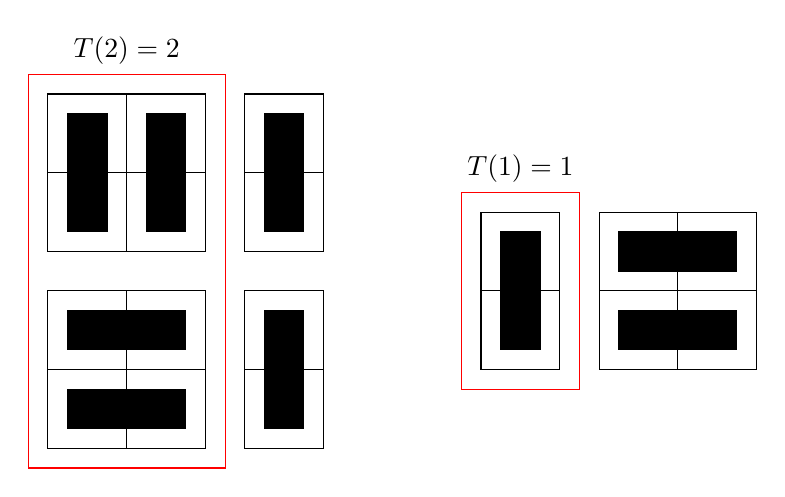
\begin{tikzpicture}[x=1.0cm, y=1.0cm]
        \foreach \g in {0, 2.5} {
            \foreach \y in {0,1} {
                \foreach \x in {0,1} {
                    \draw (0+\x ,0+\y+\g) rectangle ++ (1,1);
                }
            }
            \draw (2.5,0+\g) rectangle ++ (1,1);
            \draw (2.5,1+\g) rectangle ++ (1,1);
            \draw[fill, black] (2.75 ,0.25+\g) rectangle ++ (0.5,1.5);
        }

        \draw[fill, black] (0.25 ,0.25) rectangle ++ (1.5,0.5);
        \draw[fill, black] (0.25 ,1.25) rectangle ++ (1.5,0.5);

        \draw[fill, black] (0.25 ,2.5+0.25) rectangle ++ (0.5,1.5);
        \draw[fill, black] (1.25 ,2.5+0.25) rectangle ++ (0.5,1.5);

        \draw[red] (-0.25, -0.25) rectangle ++(2.5, 5);
        \path (-0.25,4.75) --  (2.25,4.75) node[midway,above,black] {$T(2)=2$};

        \draw (5.5,1) rectangle ++ (1,1);
        \draw (5.5,2) rectangle ++ (1,1);
        \draw[fill, black] (5.75 ,1.25) rectangle ++ (0.5,1.5);
        \draw[red] (5.25, 0.75) rectangle ++(1.5, 2.5);
        \path (5.25,3.25) --  (6.75,3.25) node[midway,above,black] {$T(1)=1$};

        \foreach \y in {0,1} {
            \foreach \x in {0,1} {
                \draw (7+\x ,1+\y) rectangle ++ (1,1);
            }
        }
        \draw[fill, black] (7.25 ,1.25) rectangle ++ (1.5,0.5);
        \draw[fill, black] (7.25 ,2.25) rectangle ++ (1.5,0.5);

    \end{tikzpicture}
\end{center}
\[T(3) = 3 = 2 + 1 = T(2) + T(1)\]

规律初现!再验证 $n = 4$:向 $T(3)$ 的每种密铺添加竖直骨牌,或向 $T(2)$ 的每种密铺添加两块水平骨牌,即可得到 $T(4)$ 的\emph{所有}密铺:

\begin{center}
    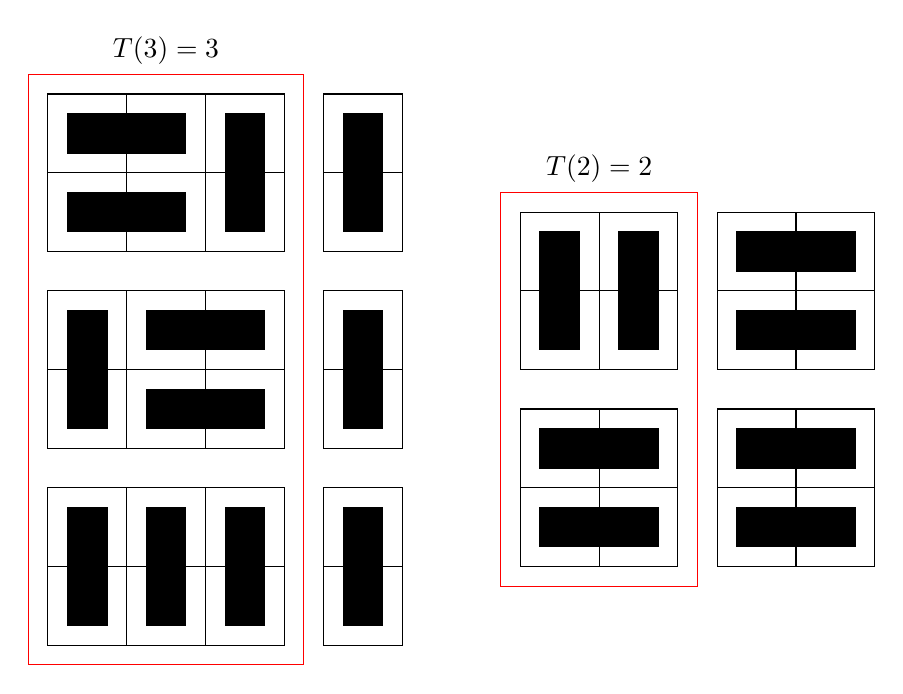
\begin{tikzpicture}[x=1.0cm, y=1.0cm]
        \foreach \g in {0, 2.5, 5} {
            \foreach \y in {0,1} {
                \foreach \x in {0,1,2} {
                    \draw (0+\x ,0+\y+\g) rectangle ++ (1,1);
                }
            }

            \draw (3.5,\g+0) rectangle ++ (1,1);
            \draw (3.5,\g+1) rectangle ++ (1,1);
            \draw[fill, black] (3.75 ,\g+0.25) rectangle ++ (0.5,1.5);
        }
        \draw[fill, black] (0.25 ,0.25) rectangle ++ (0.5,1.5);
        \draw[fill, black] (1.25 ,0.25) rectangle ++ (0.5,1.5);
        \draw[fill, black] (2.25 ,0.25) rectangle ++ (0.5,1.5);

        \draw[fill, black] (0.25 ,2.75) rectangle ++ (0.5,1.5);
        \draw[fill, black] (1.25 ,2.75) rectangle ++ (1.5,0.5);
        \draw[fill, black] (1.25 ,3.75) rectangle ++ (1.5,0.5);

        \draw[fill, black] (2.25 ,5.25) rectangle ++ (0.5,1.5);
        \draw[fill, black] (0.25 ,5.25) rectangle ++ (1.5,0.5);
        \draw[fill, black] (0.25 ,6.25) rectangle ++ (1.5,0.5);

        \draw[red] (-0.25, -0.25) rectangle ++(3.5, 7.5);
        \path (-0.25,7.25) --  (3.25,7.25) node[midway,above,black] {$T(3)=3$};


        \foreach \g in {0, 2.5} {
            \foreach \y in {0,1} {
                \foreach \x in {0,1} {
                    \draw (6+\x ,1+\y+\g) rectangle ++ (1,1);
                }
            }
            \foreach \y in {0,1} {
                \foreach \x in {0,1} {
                    \draw (8.5+\x ,1+\y+\g) rectangle ++ (1,1);
                }
                \draw[fill, black] (8.75 ,1.25+\g+\y) rectangle ++ (1.5,0.5);
            }
           
        }

        \draw[fill, black] (6.25 ,1.25) rectangle ++ (1.5,0.5);
        \draw[fill, black] (6.25 ,2.25) rectangle ++ (1.5,0.5);

        \draw[fill, black] (6.25 ,3.5+0.25) rectangle ++ (0.5,1.5);
        \draw[fill, black] (7.25 ,3.5+0.25) rectangle ++ (0.5,1.5);

        \draw[red] (5.75, 0.75) rectangle ++(2.5, 5);
        \path (5.75,5.75) --  (8.25,5.75) node[midway,above,black] {$T(2)=2$};
        
    \end{tikzpicture}
\end{center}
\[T(4) = 5 = 3 + 2 = T(3) + T(2)\]

需要注意的是,此方式不会产生重复密铺。(仔细思考为何能保证唯一性?)由此可直接推出 $T(4) = T(3) + T(2)$。

此外,上述论证具有普适性。对于任意 $n$,观察棋盘最右侧:若为竖直骨牌,则密铺源于 $2 \times (n - 1)$ 棋盘;若为水平骨牌对,则源于 $2 \times (n-2)$ 棋盘。因此对所有满足条件的 $n$ 有:
\[T(n) = T(n - 1) + T(n - 2)\]
哪些 $n$ 值适用?请记住,我们必须单独分析 $T(1)$ 和 $T(2)$;因此上述公式不适用于 $n=1$ 和 $n=2$,我们必须添加限制条件 $n \ge 3$ 才能使上面公式成立。

据此可轻松计算任意 $n$ 对应的 $T(n)$,甚至可编程实现。但正是\emph{归纳}论证——对模式的细致观察及其成因的透彻分析——使我们得出最终结论。本例中,$T(n)$ 的值依赖于前两项 $T(n-1)$ 和 $T(n-2)$,这在前文示例中\emph{未曾}出现,这暗示了更深层的机制。是否察觉此前的归纳定义与多米诺骨牌类比在此失效?如何修正类比以解释此情况?思考一下这些问题,然后再继续阅读。我们将在下一个示例之后深入讨论它们。

顺便一提,你是否注意到此数列的特别之处?你还知道其他类似的数列吗?思考一下吧……


% !TeX root = ../../../book.tex
\subsection{制胜策略}

这个例子将是我们第一个\emph{无需}证明数值公式的归纳问题!这似乎很奇怪,但正如即将看到的那样,这却是一个事实。实际上在数学中,这比你想象的更常见:一个问题或数学对象可能存在某些潜在的归纳结构,但却不依赖代数或算术的内容。

事实上,我们将讨论一个\emph{游戏}。就是通常意义上的游戏——有两个玩家必须遵守的规则,并且有明显的赢家和输家——同时也是数学意义上的游戏,我们可以使用数学符号来制定规则和游戏情境,并以抽象的方式讨论\emph{策略}。我们甚至可以\emph{解}这个游戏。这与棒球比赛非常不同。

现在让我们讨论一下这个游戏的规则,我们暂时将其称为``取石子''。有两个玩家,称为 $P_1$ 和 $P_2$。玩家 $P_1$ 先行。玩家面前的桌子上有两堆石子,每堆正好有 $n$ 个石子,其中 $n$ 是某个自然数。(为了区分游戏的不同版本,当每堆石子有 $n$ 个石子时,我们会说玩家正在``玩 $T_n$''。)在每个玩家的回合中,他们可以从\emph{任意}一堆中取走\emph{任意}数量的石子。但不能同时从两堆石子中取石子。取走\emph{最后}一颗石子的玩家\emph{获胜}。

试着跟朋友玩一下这个游戏。使用硬币或糖果当石子。再试着切换一下角色,你先作为 $P_1$,然后再作为 $P_2$。尝试制定一个获胜\emph{策略},一种最大化获胜机会的游戏方法。尝试猜测不同的 $n$ 值下会发生什么。谁``应该''获胜?你能\emph{证明}吗?说真的,在继续阅读我们的分析之前,先玩玩这个游戏并尝试证明一些结论。你可能会对自己所取得的成就感到惊讶!

与其他示例一样,让我们使用 $n$ 的一些较小值来弄清楚到底发生了什么,然后再尝试进行泛化。当 $n = 1$ 时,这个游戏相当愚蠢。$P_1$ 必须取走其中一堆中唯一的石子,然后 $P_2$ 取走另一堆中唯一剩余的石子。因此,$P_2$ 胜。(请注意,无论 $P_1$ 选择两堆中的哪一堆,$P_2$ 总是会得到另一堆。我们可以说``不失一般性'', $P_1$ 选择左边这堆,因为无论选择哪一堆都无关紧要;情况是等价的,所以为了方便具体讨论,我们不妨说是左边这堆。后面讨论数理逻辑时,我们也会深入探讨``不失一般性''这一思想。)


\begin{center}
    \begin{tikzpicture}[line width=0.5mm]
        \foreach \n in {0, 1}{
            \node at (\n, 0)[circle,fill,inner sep=8pt, anchor=west]{};
            \draw (\n, -1) -- +(0.8, 0);
        }
        \draw[-latex] (2.5, -0.4) -- +(2, 0) node[midway,above]{$P_1$ 回合};
        \draw (5, -1) -- +(0.8, 0);
        \node at (6, 0)[circle,fill,inner sep=8pt, anchor=west]{};
        \draw (6, -1) -- +(0.8, 0);
        \draw[-latex] (7.5, -0.4) -- +(2, 0) node[midway,above]{$P_2$ 回合};
        \draw (10, -1) -- +(0.8, 0);
        \draw (11, -1) -- +(0.8, 0);
        \path (10, -0.4) -- +(2, 0) node[midway,above]{$P_2$ 胜!};
    \end{tikzpicture}
\end{center}

当 $n = 2$ 时,可能会出现几种情况。思考 $P_1$ 可能采取的行动。同样地,$P_1$ 可能选择左堆也可能选择右堆,但因为最终结果是相同的,并且我们可以交换这两堆,所以我们可以说(不失一般性)$P_1$ 从左堆取走若干石子。具体是多少?可能是一颗石子也可能是两颗石子。让我们分别检验每种情况。

\begin{center}
    \begin{tikzpicture}[line width=0.5mm]
        \foreach \x in {0, 1}{
            \node at (\x, 0)[circle,fill,inner sep=8pt, anchor=west]{};
            \node at (\x, 1)[circle,fill,inner sep=8pt, anchor=west]{};
            \draw (\x, -1) -- +(0.8, 0);
        }
        \draw[-latex] (2.5, -0.4) -- +(2, -0.6);
        \draw[-latex] (2.5, 0.6) -- +(2, 0.6);
        \node[anchor=west] at(2.5,0) {$P_1$ 回合};
        \foreach \delta in {1, -2}{
            \foreach \n in {0, 1}{
                \draw (5+\n, \delta) -- +(0.8, 0);
                \node at (6, \delta+1+\n)[circle,fill,inner sep=8pt, anchor=west]{};
            }
        }
        \node at (5, -1)[circle,fill,inner sep=8pt, anchor=west]{};
        \draw[-latex] (7.5, 2) -- +(2, 0) node[midway,above]{$P_2$ 回合};
        \draw[-latex] (7.5, -1) -- +(2, 0) node[midway,above]{$P_2$ 回合};
        \draw (10, 1) -- +(0.8, 0);
        \draw (11, 1) -- +(0.8, 0);
        \path (10, 1.6) -- +(2, 0) node[midway,above]{$P_2$ 胜!};
        \path (10, -1.4) -- +(2, 0) node[midway,above]{???};
    \end{tikzpicture}
\end{center}

如果 $P_1$ 取走两颗石子,$P_2$ 应该如何应对呢?$P_2$ 可以取走另一堆从而获胜,所以 $P_1$ 一开始就不应该采取这一行动。不过,可能 $P_1$ 脑子不清什么的,而且我们需要考虑所有可能的情况来全面分析这场比赛。因此,在这种情况下(上图中的上半行)$P_2$ 获胜。好吧,这就是简单的情况。

如果 $P_1$ 只从左边一堆石子(上图中的下半行)中取走一颗石子怎么办?$P_2$ 应该如何应对?我们现在有几种选择:

\begin{itemize}
    \item 如果 $P_2$ 从左边一堆石子中取走另一颗石子……那么,$P_2$ 取走另一堆全部石子,$P_1$ 获胜。
    \item 如果 $P_2$ 从右边一堆石子中取走全部两颗石子……那么,$P_1$ 取走左边一堆中的最后一颗石子,$P_1$ 获胜。
    \item 然而,如果 $P_2$ 只从右边一堆石子中取走一颗石子……
\end{itemize}

\begin{center}
    \begin{tikzpicture}[line width=0.5mm]
        \foreach \g in {0, 5, 10} {
            \foreach \x in {0, 1} {
                \node at (\x+\g, 0)[circle,fill,inner sep=8pt, anchor=west]{};
                \draw (\x+\g, -1) -- +(0.8, 0);
            }
        }
        \node at (0, 1)[circle,fill,inner sep=8pt, anchor=west]{};
        \node at (1, 1)[circle,fill,inner sep=8pt, anchor=west]{};
        \draw[-latex] (2.5, -0.4) -- +(2, 0) node[midway,above]{$P_1$ 回合};

        \node at (6, 1)[circle,fill,inner sep=8pt, anchor=west]{};
        \draw[-latex] (7.5, -0.4) -- +(2, 0) node[midway,above]{$P_2$ 回合};
    \end{tikzpicture}
\end{center}
现在我们遇到了与 $T_1$ 完全相同的情况,我们已经对此进行了分析!这次又是 $P_1$ 先走的,所以我们知道会发生什么:无论如何 $P_2$ 都会获胜。如果你是玩家 $P_2$,这显然是最好的应对:\emph{无论} $P_1$ \emph{如何行动},你都会赢!

退一步,让我们思考一下这表明了什么:无论 $P_1$ 首先采取什么行动(从任一堆中取走一个或两个石子),$P_2$ 都可以做出\emph{某个可能的回应,保证} $P_2$ 总会获胜,无论 $P_1$ 随后采取什么回应。哇,$P_2$ 稳坐钓鱼台!让我们看看其他 $n$ 值的情况下是否会发生同样的事情。

当 $n = 3$ 时,我们将再次假设(不失一般性)玩家 $P_1$ 从左边石子堆上取石子。他可以取走一颗、两颗或三颗石子:

\begin{itemize}
    \item 如果 $P_1$ 取走全部三颗,那么 $P_2$ 就会完全拿走另一堆并获胜。
    \item 如果 $P_1$ 取走两颗石子……那么 $P_2$ 应该做什么呢?
\end{itemize}
取完左边一堆是愚蠢的(因为 $P_1$ 可以取走整个右边一堆从而获胜),而取走整个右边一堆也同样愚蠢(因为 $P_1$ 可以取走整个左边一堆从而获胜),所以需要介于两者之间。现在,如果 $P_2$ 仅从右侧一堆石子中取走一颗石子,请注意 $P_1$ 可以采用相同的动作做出回应;从而使得两堆石子都只剩下一颗,但先手互换了。在这种情况下,$P_2$ 先行,根据我们之前的分析,$P_2$ 肯定会输。因此这是糟糕的策略!

\begin{center}
    \begin{tikzpicture}[line width=0.5mm]
        \foreach \g in {0, 5, 10, 15}{
            \foreach \x in {0, 1}{
                \node at (\x+\g, 0)[circle,fill,inner sep=8pt, anchor=west]{};
                \draw (\x+\g, -1) -- +(0.8, 0);
            }
        }
        \foreach \x in {0, 1, 6}{
            \foreach \y in {0, 1}{
                \node at (\x, \y)[circle,fill,inner sep=8pt, anchor=west]{};
                \node at (\x, \y+1)[circle,fill,inner sep=8pt, anchor=west]{};
            }
        }

        \node at (11, 1)[circle,fill,inner sep=8pt, anchor=west]{};

        \draw[-latex] (2.5, -0.4) -- +(2, 0) node[midway,above]{$P_1$ 回合};
        \draw[-latex] (7.5, -0.4) -- +(2, 0) node[midway,above]{$P_2$ 回合};
        \draw[-latex] (12.5, -0.4) -- +(2, 0) node[midway,above]{$P_1$ 回合};
        \path (15, 0.6) -- +(2, 0) node[midway,above]{$P_1$ 胜!};
    \end{tikzpicture}
\end{center}

让我们再试一次。如果 $P_2$ 从右边一堆石子中取走两颗石子……瞧!现在,我们每堆中只有一颗石子,$P_1$ 先行,所以我们知道  $P_1$ 一定会输。$P_2$ 再次完胜!

\begin{center}
    \begin{tikzpicture}[line width=0.5mm]
        \foreach \g in {0, 5, 10}{
            \foreach \x in {0, 1}{
                \node at (\x+\g, 0)[circle,fill,inner sep=8pt, anchor=west]{};
                \draw (\x+\g, -1) -- +(0.8, 0);
            }
        }
        \foreach \x in {0, 1, 6}{
            \foreach \y in {0, 1}{
                \node at (\x, \y)[circle,fill,inner sep=8pt, anchor=west]{};
            }
        }
        \draw[-latex] (2.5, -0.4) -- +(2, 0) node[midway,above]{$P_1$ 回合};
        \draw[-latex] (7.5, -0.4) -- +(2, 0) node[midway,above]{$P_2$ 回合};
        \path (10, 0.6) -- +(2, 0) node[midway,above]{$P_2$ 胜!};
    \end{tikzpicture}
\end{center}

思考一下 $n = 4$ 的情况,你会发现完全相同的分析再次出现。你会考虑另一种可能性:玩家 $P_1$ 可以从左边一堆石子中取走一颗、两颗、三颗或四颗。不过,无论 $P_1$ 怎么做,你都会发现 $P_2$ 可以在另一堆上\emph{模仿}相同的动作,将整个游戏简化为之前的\emph{较小}版本,从而保证 $P_2$ 一定获胜!看起来 $P_2$ 一直处于主导地位,因为他可以对 $P_1$ 的任何行为做出回应,在另一堆上做出相同的动作。无论 $P_1$ 做什么,$P_2$ 总会做出回应,这意味着 $P_2$ 一定获胜,无论 $P_1$ 随后的动作是什么。从这个意义上讲,我们说``$P_2$ 有制胜策略''。$P_2$ 有一个清晰且可描述的方法来评估比赛局势并选择特定的行动来\emph{保证获胜}。

我们要如何证明这一点?如何应用本章的归纳法?目前可能很难看出来。我们在这里到底要证明什么?对这个问题的类比中,多米诺骨牌或阶梯是什么?在你开动脑筋思考这个例子时,你应该意识到以下几点:归纳法并不总是与代数式有关;归纳法代表某种``构建''结构,较大的情况依赖于较小的情况;我们必须证明一些初始事实,然后论证如何化简任意更大事实,使其依赖于先前的事实。这才是多米诺骨牌类比的真正目的。碰巧的是,这个类比可以很好地解释某些归纳问题(但不是全部),并且是可视化的,令人印象深刻。但它并不完全适用于\emph{所有}情况。

回顾本章的四个例子,思考它们有何相似之处和不同之处。 尝试使用一些更好的术语(也许是你自己发明的)对数学归纳法进行更精确的数学描述。(这里的意思是比直观的类比更好。你会惊讶地发现,在不真正知道自己``应该''说什么的情况下,你竟然能够很好地描述归纳法,并且在这个过程中你会学到很多东西!)在适当的时候,我们会对数学归纳法及其各种形式进行严格的陈述和证明。与此同时,我们需要探索数学的一些其他领域,以建立必要的语言、符号和知识,以便回过头解决这个问题。不过,在开始之前,我们应该了解一下数学归纳法的一些有用的应用。


% !TeX root = ../../../book.tex
\subsection{习题}

\subsubsection*{温故知新}

以口头或书面的形式简要回答以下问题。这些问题全都基于你刚刚阅读的内容,如果忘记了具体定义、概念或示例,可以回顾相关内容。确保在继续学习之前能够自信地作答这些问题,这将有助于你的理解和记忆!

\begin{enumerate}[label=(\arabic*)]
    \item 如何\emph{归纳}这两个例子?它们与立方体、直线的例子在哪些方面相似?在哪些方面不同?
    \item 对于多米诺骨牌密铺问题,计算 $T(n)$ 需要知道前几项值?
    \item $T(n) = T(n - 1) + T(n - 2)$ 与 $T(n + 2) = T(n + 1) + T(n)$ 有什么区别?
    \item 取石子游戏的必胜策略是什么?请与不了解策略的朋友试玩,并采用玩家 $P_2$ 的必胜策略。观察你每次获胜时对方的反应如何?对方是否开始察觉这一策略?
\end{enumerate}

\subsubsection*{小试牛刀}

尝试解答以下问题。这些题目需动笔书写或口头阐述答案,旨在帮助你熟练运用新概念、定义及符号。题目难度适中,确保掌握它们将大有裨益!

\begin{enumerate}[label=(\arabic*)]
    \item $T(5)$ 的值是多少?能否画出所有密铺方案?
    \item 分析两堆各 $4$ 颗石子的取石子游戏:玩家 $P_2$ 是否总有必胜策略?
    \item \textbf{挑战题:}若使用\emph{三堆}等量石子进行游戏,会如何发展?能否为任意一方找到必胜策略?不妨与朋友实际对弈,观察结果!
    \item 探索\emph{斐波那契数列}:它与多米诺骨牌密铺问题中的数列 $T(n)$ 有何关联?
\end{enumerate}

\newpage
% !TeX root = ../../../book.tex
\section{应用}

% !TeX root = ../../../book.tex
\subsection{递归程序}\label{sec:section2.5.1}

数学归纳法背后的概念在计算机科学中有着广泛应用。回想我们推导 $\sum_{k=1}^{n}k^2$ 公式的过程:一旦找到用较小立方和及剩余项表示立方数的方法,就会反复进行替换,直到抵达最初观察到的``最简''情况——即计算起点 $2^3=1+3+3+1$。递归编程正是运用了这一思想:通过确定``大''问题如何依赖``小''案例来简化问题,直至达到已知的简单案例。

此类技术的经典示例是计算\emph{阶乘} $n!$ 的代码,其定义为前 $n$ 个自然数的乘积:
\[n! = 1 \cdot 2 \cdot 3 \dots (n - 1) \cdot n\]
这个定义对人类而言直观易懂,但指导计算机执行该乘积却并非易事(尝试思考:如何在代码中表达``持续执行直至达到 $n$''?)。实际上,更有效的函数编程方法以及对数学归纳定义的建模,是让程序\emph{递归调用自身}直至``最简''情况。对于阶乘而言,该情况即 $1! = 1$。对于任意其他 $n$ 值,可反复应用关系:
\[n! = (n - 1)! \cdot n\]
来计算 $n!$。以下\emph{伪代码}体现了这一思想:

\begin{verbatim}
    factorial(n):
        if n = 1
            return 1
        else
            return n * factorial(n-1)
    end
\end{verbatim}

我们已知 $1! = 1$,若需计算此值,将直接返回正确结果。对于任意 $n > 1$,程序会调用\emph{自身}:``请计算 $(n-1)!$,然后乘以 $n$ 得到答案。''为计算 $(n-1)!$,程序再次检查输入是否为 $1$;若不为 $1$,则继续调用自身:``请计算 $(n-2)!$,然后乘以 $(n-1)$。''此过程持续至程序返回 $1! = 1$。随后,程序便能计算 $2! = 1 \times 2$,进而 $3! = 2! \times 3$,依此类推,最终得到 $n! = (n - 1)! \times n$。

\clearpage

递归编程的另一个经典例子是\emph{斐波那契数列}。你可能在数学课上见过这个数列(事实上,我们在上一节讨论多米诺骨牌密铺时提到过它),或者听说过它以有趣而奇妙的方式出现在自然界中——该数列最早由意大利比萨数学家莱昂纳多·斐波那契 (Leonardo Fibonacci) 在研究兔子种群增长时``发现''。斐波那契数列的前两项均为 $1$,后续每一项都定义为前两项之和。若用 $F(n)$ 表示第 $n$ 个斐波那契数,则有:
\[F(1) = 1 \text{\ 且\ }F(2) = 1, \text{ 对于任意\ } n \ge 3, F(n) = F(n - 1) + F(n - 2)\]
那么,$F(5)$ 等于多少?$F(100)$ 或 $F(10000)$ 呢?递归程序可以轻松解决这个问题。思路一致:当函数遇到基本情况 $F(1)$ 或 $F(2)$ 时,直接返回 $1$;否则,递归调用自身计算前两项并求和。阅读以下伪代码并思考其工作原理:若用此程序计算 $F(10)$,过程会如何展开?

\begin{verbatim}
    Fibonacci(n):
        if n = 1 or n = 2
            return 1
        else
            return Fibonacci(n-1) + Fibonacci(n-2)
    end
\end{verbatim}

该程序与 \verb|factorial| 函数思路相似(通过递归调用计算更小规模的问题直至达到已知解),但蕴含更深层的机制。若输入 $n = 10$,程序发现结果未知,将调用自身计算 \verb|Fibonacci(9)| 和 \verb|Fibonacci(8)|。每次调用遇到未知值时,又会触发新的递归计算——例如为求 $F(9)$ 需计算 $F(8)$ 和 $F(7)$,而为求 $F(8)$ 又需计算 $F(7)$ 和 $F(6)$。这导致相同输入值被多次重复计算。

请比较 \verb|Fibonacci| 与 \verb|factorial| 程序,思考它们如何体现归纳过程的核心思想。两者是否采用类似策略?与介绍数学归纳法时用到的``多米诺骨牌''类比有何关联?不妨将骨牌 $n$ 的``事实''视为 $n!$ 的正确计算或 $F(n)$ 的值,这个类比在两种情况下如何成立?所有骨牌是否必然倒下?在继续阅读之前,请带着这些问题深入思考——其背后蕴藏着强大的数学基础。

\clearpage


% !TeX root = ../../../book.tex
\subsection{汉诺塔}

我们休息一下,玩个游戏吧。其实不完全是休息,因为从某种意义上来说,这是一个\emph{归纳}游戏,所以是完全相关的。但好歹是个游戏!\emph{汉诺塔}是一个非常受欢迎的智力游戏,部分原因在于它的规则和设备都很简单。不过解决这个问题却一点也不简单!

想象一下,我们有三个垂直的杆和三个不同尺寸(\textcolor{blue}{蓝色}、\textcolor{olivegreen}{绿色}和\textcolor{red}{红色})的圆盘,彼此叠放在一起,如下所示:

\begin{center}
    \begin{tikzpicture}[line width=4mm,line cap=round,xscale=3,brown!30]
        \def\sequence{3/1,2/1,1/1}
        % init colors
        \foreach[count=\j] \c in {red,olivegreen,blue}
            \gset col[\j]={\c};
        \edef\numdisks{\j}
        % init positions and draw support
        \foreach \j in {1,2,3}{
            \gset pos[\j]=0
            \draw (\j,-.4) -- +(0,3);
        }
        \draw (.5,-.4) -- +(3,0);

        % draw
        \foreach[count=\k] \i/\j in \sequence{
            \edef\delta{\i*0.4/3}
            \draw[draw={\get col[\i]}](\j-\delta,\get pos[\j]) -- (\j+\delta,\get pos[\j]);
            \ginc pos[\j]+={.4}
        }
    \end{tikzpicture}
\end{center}
目标是通过遵循以下规则将所有三个圆盘移动到另一根杆上(无论是中间的还是右边的,都没关系):

\begin{enumerate}
    \item 每次移动只能将一根杆子顶部的一个(且\emph{仅有}一个)圆盘,移动到另一根杆子的顶部,
    \item 任何圆盘不能放置在比它小的圆盘之上。
\end{enumerate}
就这些!两条简单的规则,但却是一个很难的游戏。尝试用一些硬币或扑克牌或任何你手边的东西来模拟这个游戏。(你甚至可以在一些游戏商店购买汉诺塔套装。)你能解决这个问题吗? 你花了多少步?你的解决方案是``最好''的吗?为什么是或者为什么不是呢?

我们提到过这是一个归纳游戏,所以让我们探讨一下这个想法。我们想要解决这个难题需要多少步(其中一步表示一个圆盘从一根杆移动到另一根杆),更具体地说,确定解决这个难题所需的\emph{最小可能步数}。对于三个圆盘的问题,如果我们愿意的话,完全可以不断地在两根杆之间来回移动最小圆盘并产生 $100$ 次移动,然后再解决它,但这肯定不是最好的方法,对吗?假设我们找到了一种在一定步数内解决问题的方法;我们如何证明我们使用的步数是最小可能步数?

为了解决这个问题,我们想\emph{递归地}分解解题方法。在此过程中,我们实际上要回答一个更普遍的问题:解决 $3$ 根杆上 $n$ 个圆盘的汉诺塔问题需要的最小移动步数是多少?我们仅用 $3$ 个圆盘提出了问题,是为了便于为你提供一个具体的版本供你思考和使用,但我们可以通过深入思考来回答这个更普遍的问题。为了确保我们理解一致,我们将向你展示如何解决具有 $3$ 个圆盘的问题:

\begin{center}
    \begin{tikzpicture}[line width=2.6mm,line cap=round,xscale=1.5,yscale=0.5,brown!30]
        \def\sequencelist{{3/1,2/1,1/1}, {3/1,2/1,1/3}, {3/1,2/2,1/3}, {3/1,2/2,1/2}, {3/3,2/2,1/2}, {3/3,2/2,1/1}, {3/3,2/3,1/1}, {3/3,2/3,1/3}}
        % init colors
        \foreach[count=\j] \c in {red,olivegreen,blue}
            \gset col[\j]={\c};
        \edef\numdisks{\j}
        \foreach[count=\n] \sequence in \sequencelist {
            % init positions and draw support
            \foreach \j in {1,2,3}{
                \gset pos[\j]=0
                \draw (\j,-0.4-5*\n) -- +(0, 3);
            }
            \draw (0.5,-0.52-5*\n) -- +(3,0);
            % draw
            \foreach[count=\k] \i/\j in \sequence{
                \edef\delta{\i*0.4/3}
                \draw[draw={\get col[\i]}](\j-\delta,\get pos[\j]-5*\n) -- (\j+\delta,\get pos[\j]-5*\n);
                \ginc pos[\j]+={0.52}
            }
        }
        \node[black,left] at (0,-5.52){开始};
        \foreach \m in {1, ..., 7} {
            \node[black,left] at (0,-5.52-5*\m){第 \m 步};
        }   
    \end{tikzpicture}
\end{center}

请注意,最大的圆盘对于大多数解决方案来说基本上是``无关''的。由于我们可以在其上面放置任何其他圆盘,因此我们需要做的就是通过将其他圆盘移动到不同的杆上来``露出''该圆盘,将最大的圆盘移动到唯一的空杆上,然后再将其他圆盘移到大圆盘上。本质上,我们执行相同的过程(将两个较小的圆盘从一根杆移动到另一根杆)两次,在两次之间,我们将大圆盘从一根杆移动到另一根杆。如果最大的圆盘根本不存在,那么我们实际做的就是 $2$ 个圆盘的题目,只是做了两次!(仔细思考这一点,确保你理解了上面这段话。假装大的\textcolor{blue}{蓝色}圆盘不存在,操作一遍上图中步骤。)

这表明解决 $3$ 盘问题的方法涉及解决 $2$ 盘问题的两次迭代,中间有一次额外的移动(移动最大的圆盘)。一般来说,这表明了解决该问题的\emph{递归}过程。为了最优地解决 $n$ 盘问题,我们只需遵循解决 $(n - 1)$ 盘问题的最优过程,用一步移动最大的第 $n$ 个圆盘,然后再次求解 $(n - 1)$ 盘问题。

现在我们对如何最优地解决这个问题有了一些了解,让我们确定该过程需要几步。认识到解决这个问题需要使用\emph{递归}算法,我们意识到\emph{证明}有关最佳解决方案的任何内容都需要\emph{归纳法}。因此,我们需要为我们的多米诺骨牌线确定一个``起点'',它应该对应于问题的``最小''或``最简单''版本。对于汉诺塔问题来说,最简问题就是 $1$ 个圆盘问题。当然,这几乎不是一个``问题'',因为我们可以一步解决它,只需将唯一的圆盘从一根杆移动到另一根杆即可。如果我们令 $M(n)$ 表示解决 $n$ 盘问题所需的最少移动次数,那么我们就确定了 $M(1) = 1$。为了确定 $M(2)$,我们可以使用上面的观察结果并得到
\[\underbrace{M(2)}_{2 \text{盘问题}}= \underbrace{M(1)}_{1 \text{盘问题}}+ \underbrace{1}_{\text{移动最大盘}}+ \underbrace{M(1)}_{1 \text{盘问题}}= 1 + 1 + 1 = 3\]
接下来一定是
\[M(3) = M(2) + 1 + M(2) = 3 + 1 + 3 = 7\]
和
\[M(4) = M(3) + 1 + M(3) = 7 + 1 + 7 = 15\]
以此类推。你注意到其中的规律了吗?这些数字中的每一个都比 $2$ 的幂小 $1$,具体来说,我们注意到对于迄今为止我们所考察的每种情况,$M(n) = 2^n - 1$。需要指出的是,观察到这种规律并不等于证明了这种规律;因为它仅仅适用于前 $4$ 种情况,并不意味着这种规律会一直持续下去,而这正是归纳证明所要解决的问题。此外,认识到这种规律并``观察''到 $M(n) = 2^n - 1$ 本身就是一件了不起的事情。我们碰巧知道答案,并且可以直接找出公式。你可以尝试自己``解决''以下关系
\[M(n) = 2M(n - 1) + 1 \text{ 且 } M(1) = 1\]
看看能否推导出公式 $M(n) = 2^n -1$。这种公式比上面的关系式更好的原因在于,$M(n)$ 仅取决于 $n$,而\emph{不再}取决于之前的项(例如 $M(n-1)$)。这种关系和其他类似关系被称为\emph{递归关系},一般来说,它们可能很难解决!

我们知道如何解决这个问题,并得出 $M(n) = 2^n - 1$。不过,相关的验证工作就留给你独立完成。你可以通过检查上面等式中的一些值来做到这一点,但我们都知道这并不构成\emph{证明}。尝试通过归纳步骤来实际证明这一点!我们已经完成了大部分工作,但还需你仔细、清晰地将一切串联在一起。请记住,你应该确定每张多米诺骨牌上的``事实''是什么,确保多米诺骨牌 $1$ 会倒下,然后对多米诺骨牌 $n$ 倒下会引起多米诺骨牌 $(n+1)$ 倒下进行一般论证。试着写出这个证明。这些细节对你来说有意义吗?向朋友展示你的证明,看看他们是否理解。你还需要告诉他们其他事情或指导他们完成证明阅读?考虑解释你的方法和步骤的最佳方式,以便书面版本就足够了,而不必添加任何口头解释。思考\emph{解释}你的方法和步骤的最佳方式,确保书面版本足够清晰准确,而不必添加任何口头解释。 


% !TeX root = ../../../book.tex
\subsection{习题}

\subsubsection*{温故知新}

以口头或书面的形式简要回答以下问题。这些问题全都基于你刚刚阅读的内容,所以如果忘记了具体的定义、概念或示例,可以回去重读相关部分。确保在继续学习之前能够自信地回答这些问题,这将有助于你的理解和记忆!

\begin{enumerate}[label=(\arabic*)]
    \item 递归程序如何归纳?
    \item 汉诺塔的归纳结构是什么?在解决 $3$ 盘问题时,我们在哪里解决了 $2$ 盘问题?
\end{enumerate}

\subsubsection*{小试牛刀}

尝试回答以下问题。这些题目要求你实际动笔写下答案,或(对朋友/同学)口头陈述答案。目的是帮助你练习使用新的概念、定义和符号。题目都比较简单,确保能够解决这些问题将对你大有帮助!

\begin{enumerate}[label=(\arabic*)]
    \item 按照伪代码 \verb|factorial| 的步骤计算 $5!$。
    \item 按照伪代码 \verb|Fibonacci| 的步骤计算 $F(5)$。
    \item 解决 $4$ 盘汉诺塔问题。确保你能以\emph{最优}步数 $2^4 - 1 = 15$ 步完成。
\end{enumerate}

\newpage
% !TeX root = ../../../book.tex
\section{总结}

我们已经看到了一些\textbf{归纳证明}的例子。我们意识到我们正在解决的一些问题使用了类似的证明风格,并探索了几个例子来了解这些证明中可能出现的不同问题。具体来说,我们看到归纳证明\emph{并不}总是证明求和公式或方程:归纳证明适用于\emph{任何}依赖于该事实的``先前事实''的情况。这导致我们从数学角度对归纳法的工作原理进行了类比。目前,我们最喜欢用``多米诺骨牌类比''来思考归纳法,但我们接下来的主要目标之一是严格\emph{陈述}和\emph{证明}归纳法原理。现在,让我们对这种类型的证明进行大量练习。这就是本章习题的目的。稍后,一旦我们将归纳正式化,我们能会更好地使用归纳法,并且我们会对这一概念有更透彻的理解!

\newpage
% !TeX root = ../../../book.tex
\section{本章习题}

以下是一些问题,帮助你熟悉归纳式证明。我们不需要完全严格的证明,只要你能很好地描述过程并写下步骤即可。等我们掌握了数学归纳原理 (PMI) 和相应的证明策略后,再回头来严格证明这些问题。

\begin{exercise} \label{exc:exercises2.7.1}
    证明以下求和公式对于每个自然数都成立,对于 $n=0$ 也成立。
    \[\sum_{i=0}^{n}2^i=2^{n+1}-1\]
    后续问题:用这个结果来说明在 $2^n$ 支球队的单赛淘汰赛中需要进行多少场比赛才能确定获胜者。(例如,NCAA 疯狂三月锦标赛就使用这种赛制,其中 $n = 6$。)
\end{exercise}

\begin{exercise}
    证明对于每个大于等于 $2$ 的自然数 $n$, $3^n \ge 2^{n+1}$。
\end{exercise}

\begin{exercise}
    对于哪些自然数 $n$,下列不等式成立?先陈述结论,然后再证明它。
    \begin{enumerate}
        \item $2^n \ge (n + 1)^2$
        \item $2^n \ge n!$
        \item $3^{n+1} > n^4$
        \item $n^3 + (n + 1)^3 > (n + 2)^3$
    \end{enumerate}
\end{exercise}

\begin{exercise}
    \textbf{末日游戏}:两名玩家轮流从日历中命名日期。每一回合中,玩家可以增加月份或日期,但不能同时增加。起始位置为 1 月 1 日,说出 12 月 31 日的人获胜。确定第一个玩家的必胜策略。
    例如,玩家 1 获胜的一系列动作如下:
    \begin{itemize}
        \item 玩家 1: 1 月 10 日;
        \item 玩家 2: 3 月 10 日;
        \item 玩家 1: 8 月 10 日;
        \item 玩家 2: 8 月 25 日;
        \item 玩家 1: 8 月 28 日;
        \item 玩家 2: 11 月 28 日;
        \item 玩家 1: 11 月 30 日;
        \item 玩家 2: 12 月 30 日;
        \item 玩家 1: 12 月 31 日。
    \end{itemize}
    我们所说的\emph{必胜}策略是指玩家 1 遵循的一种游戏方法,无论玩家 2 做什么,都可以\emph{保证}获胜。
\end{exercise}

\begin{exercise}
    找到并证明\emph{几何级数}求和公式,几何级数定义如下:
    \[\sum_{i=0}^{n-1}q^i\]
    其中 $q$ 为实数,$n$ 为自然数。(提示:留意 $q = 1$ 的情况。)
\end{exercise}

\begin{exercise}
    写一个依赖于 $n$ 的句子,使得该句子对于从 $1$ 到 $99$(含)的所有 $n$ 值都为真,但当 $n = 100$ 时该句子为假。
\end{exercise}

\begin{exercise}
    下面``错误证明''证明了对于所有 $n$, $a^n=1$。请指出问题在哪里?
    \begin{spoof}
        设 $a$ 为非零实数。请注意 $a^0 = 1$。另请注意我们可以归纳地写出
        \[a^{n+1} = a^n \cdot a = a^n \cdot \frac{a^n}{a^{n-1}} = 1 \cdot \frac{1}{1} = 1\]
    \end{spoof}
\end{exercise}

\begin{exercise}
    未来社会中,只有两种面额的货币:一种价值 $3$ Brendan 的硬币,一种价值 $8$ Brendan 的硬币。还有一项全国性法令,店主只能收取可以使用这两种硬币\textbf{精确支付}的价格。

    店主可能向你收取的一杯咖啡的法定价格是多少?
    
    \textbf{提示:}尝试一些较小的值,看看会发生什么。
\end{exercise}

\begin{exercise}
    对于某个任意自然数 $n$,考虑大小为 $2^n \times 2^n$ 的棋盘。从棋盘上移除\textbf{任意}一个方格。 是否可以用 L 形三联骨牌来密铺剩余的方格?

    如果你的答案是肯定的,请证明这一点。

    如果您的答案是否定的,请提供反例论证。(也就是说,找到一个 $n$ 使得任何方法都无法密铺棋盘,并说明为什么会出现这种情况。)
\end{exercise}

\begin{exercise}
    考虑一个 $n \times n$ 的正方形网格。该网格内存在多少个任意大小的子方格?例如,当 $n = 2$ 时,答案为 $5$:有 $4$ 个$1 \times 1$ 方格和 $1$ 个 $2 \times 2$ 方格。找到你的答案的公式并尝试证明它是正确的。
\end{exercise}

\begin{exercise}
    证明,在至少有 $2$ 人的队列中,如果第一个人是女性,最后一个人是男性,那么在队列的某个位置一定存在一个男性紧邻女性身后。
\end{exercise}

\begin{exercise}
    对于每个自然数 $n$,证明 $n^3 - n$ 是 3 的倍数。
\end{exercise}

\begin{exercise}
    \textbf{二进制 $n$ 元组}是由 \verb|0| 和 \verb|1| 组成的有序字符串,字符串中共有 $n$ 个数字。提供一个\emph{归纳论证}来解释为什么有 $2^n$ 个可能的二进制 $n$ 元组。
\end{exercise}

\begin{exercise}
    回想一下,\textbf{斐波那契数}是通过设 $f_0 = 0$ 和 $f_1 = 1$,然后对于每个 $n \ge 2$,设 $f_n = f_{n-1} + f_{n-2}$ 来定义的。这会产生序列 $0, 1, 1, 2, 3, 5, 8, 13, 21, 34, \dots$

    你可能不知道,斐波那契数列也有\emph{封闭形式};也就是说,除了上面给出的常规递归定义外,还有一个特定\emph{公式}来定义它。那就是:
    \[f_n = \frac{1}{\sqrt 5}\Bigg[\Bigg(\frac{1+\sqrt 5}{2}\Bigg)^n - \Bigg(\frac{1-\sqrt 5}{2}\Bigg)^n\Bigg]\]
    证明该公式对于所有 $n \ge 0$ 都正确。
\end{exercise}

\begin{exercise}
    再次考虑斐波那契数 $f_n$,证明以下内容:
    \begin{enumerate}
        \item $\displaystyle{\sum_{i=0}^{n}f_i = f_{n+2} - 1}$
        \item $\displaystyle{\sum_{i=0}^{n}f_i^2 = f_n \cdot f_{n+1}}$
        \item $\displaystyle{f_{n-1} \cdot f_{n+1} - f_n^2 = (-1)^n}$
        \item $\displaystyle{f_{m+n} = f_n \cdot f_{n+1} + f_{m-1} \cdot f_n}$
        \item $\displaystyle{f_n^2 + f_{n+1}^2 = f_{2n+1}}$
    \end{enumerate}
\end{exercise}

\begin{exercise}
    尝试提供一个归纳论证来解释为什么每个 $n ≥ 2$ 的自然数都可以写成质数的乘积。你能证明该乘积的\emph{唯一性}吗?也就是说,你能解释为什么\emph{只有唯一一种方法}可以将自然数分解为质数吗?
\end{exercise}

\begin{exercise}
    证明
    \[\sum_{k=1}^{n} k \cdot k! = 1 \cdot 1! + 2 \cdot 2! + 3 \cdot 3! + \dots + n \cdot n! = (n+1)!-1\]
\end{exercise}

\clearpage

\begin{exercise}
    下面的``错误证明''得出所有的笔颜色都一样,问题出在哪儿?
    \begin{spoof}
        考虑一组数量为 $1$ 的笔。由于只有 $1$ 支笔,所以它的颜色肯定与自身相同。

        假设任意一组 $n$ 支笔在组内只有一种颜色。(注意:我们已经解释了为什么这个假设对于 $n = 1$ 是有效的,所以我们可以做出这个假设。)取任意一组 $n + 1$ 支笔。将它们排列在桌子上,从左到右用 $1$ 到 $n + 1$ 编号。查看其中的前 $n$ 个,即查看笔 $1,2,3, \dots , n$。这是一组 $n$ 支笔,因此根据假设,该组只有一种颜色。(我们还不知道是什么颜色。)然后,查看最后 $n$ 支笔;即查看笔 $2,3, \dots ,n+1$。这也是一组 $n$ 支笔,因此根据假设,该组也只有一种颜色。而 $2$ 号笔恰好属于这两个组。因此,无论 $2$ 号笔的颜色是什么,这也是\dotuline{两组}中每支笔的颜色。因此,所有 $n+1$ 支笔具有相同的颜色。

        根据归纳法,这表明任何一组笔,无论多少,都只有一种颜色。那么,纵观世界上有限的钢笔,我们应该只能找到一种颜色。
    \end{spoof}
\end{exercise}

\begin{exercise}
    $\star$ 这题\emph{极其难解},摘自著名数学家陶哲轩(Terence Tao)的博客(\href{https://terrytao.wordpress.com/2011/04/07/the-blue-eyed-islanders-puzzle-repost/}{详见链接})

    有一座岛屿,岛上居住着一个部落。这个部落有 $1000$ 人,有着不同颜色的眼睛。然而,他们的宗教信仰禁止他们知道自己眼睛的颜色,甚至禁止讨论这个话题;因此,每个居民都可以(并且确实可以)看到所有其他居民眼睛的颜色,但无法知道自己眼睛的颜色(不考虑反射表面)。如果部落成员确实发现了自己眼睛的颜色,那么他们的宗教信仰就会迫使他们第二天中午在村庄广场举行自杀仪式,让所有人围观。所有的部落成员都是高度逻辑和虔诚的,他们都知道其他人也是高度逻辑和虔诚的(并且他们都知道他们都知道其他人是高度逻辑和虔诚的,等等)。

    (就这个逻辑谜题而言,``高度逻辑的''意味着能够从岛民可用的信息和观察中逻辑推断出的任何结论,该岛民将自动知晓。)

    事实证明,在这 $1000$ 名岛民中,有 $100$ 人是蓝眼睛,$900$ 人是棕眼睛,尽管岛民最初并没有意识到这些统计数据(当然,他们每个人只能看到 $1000$ 名部落居民中的 $999$ 人)。

    一天,一名蓝眼睛的外国人来到岛上,并赢得了部落的完全信任。

    一天晚上,他向整个部落发表讲话,感谢他们的热情款待。

    然而,由于不了解当地习俗,这名外国人在称呼中错误地提及了眼睛的颜色,并表示\emph{在世界的其他角落看到另一个像我这样的蓝眼睛的人是多么不同寻常}。

    这种失礼(如果有的话)会对部落带来什么影响?
\end{exercise}

\newpage
% !TeX root = ../../../book.tex
\section{展望}

在本章中,我们向你介绍了\textbf{数学归纳法}的概念。我们看了一些示例,其中归纳过程指导了我们的解题思路,然后我们描述了如何通过\emph{归纳证明}来\emph{严格验证}该解题思路。凭借迄今为止我们掌握的数学技术和概念,我们必须依靠非技术性的类比来向你描述这个过程。某种程度上,这就像让朋友向你描述如何挥高尔夫球杆,即使你以前从未打过高尔夫球。当然,它们可以为你提供一些关于挥杆``感受就像是什么''的心理想象,但如果不亲自练习,你如何真正理解高尔夫挥杆的机制呢?如何学习怎样调整你的挥杆动作,或辨别一号木杆、五号铁杆和沙坑挖起杆之间的区别呢?通过研究底层机制并刻意练习,我们希望更好地理解数学归纳法,以便将来我们可以适当地使用它,识别它适用的情况,并最终学习如何使其\emph{适应}其他情况。当然,记住多米诺骨牌的类比会有助于引导我们的直觉,但我们也应该记住,这不是严格的数学。它也不能完美地描述我们讨论的其中几个例子,在这些例子中,倒下的多米诺骨牌不仅取决于紧随其后的多米诺骨牌,还取决于它之前的其他几张多米诺骨牌。

在下一章中,我们将探讨严格陈述和证明数学归纳法作为证明技术所需的一些相关概念。具体来说,我们将研究\emph{数理逻辑}的一些思想,研究如何将复杂的数学陈述和定理分解为更小的组成部分,以及如何从基本构建模块中构建起有趣且复杂的陈述。在此过程中,我们将引入一些新的符号和速记符,使我们能够将一些冗长的陈述压缩成简洁(且精确)的数学语言。有了这些之后,我们将探索一些更基本的证明策略,然后将其应用于本课程中\emph{所做的所有其他事情},包括归纳技术本身!我们还将研究\emph{集合论}的一些思想,集合论是数学的一个分支,构成了所有其他分支的基础。这对于将来组织我们的想法非常有用,而它也将帮助我们以严格的方式定义\emph{自然数}。有了这两个数学分支的一些概念和知识,我们就可以在坚实的基础上建立数学归纳法,并继续正确地使用它。